\chapter{Sperimentazione}
\label{chap:impl}

In questo capitolo viene discussa l'implementazione e l'applicazione delle metriche di Model Selection e delle tecniche di Rank Aggregation. Infine viene proposta una valutazione su dataset di benchmark e quello di SKF.

Riassumendo, questo capitolo si dividerà in:
\begin{enumerate}
	\item Definizione e implementazione delle metriche surrogate per il Model Selection e delle tecniche di Rank Aggregation
	\item Benchmark Results
	\item SKF Results
\end{enumerate}


\section{Implementazione}
Come introdotto nel capitolo \ref{chap:modelselection}, il task da risolvere e' l'implementazione di un metodo di Model Selection non supervisionato che scelga il modello o i modelli migliori dato un dataset. L'approccio scelto e' stato quello di definire delle metriche "surrogate" che siano correlate con le performance del modello e che non richiedano labels. Queste metriche sono indipendenti tra di loro ed e' necessario usarne una come candidata oppure aggregarle secondo qualche criterio. Vengono quindi proposti diversi metodologie di Rank Aggregation. Uno schema rappresentante il flusso operazione e' rappresentato in figura \ref{flow-scheme}.
\begin{figure}[t]
	\centering
	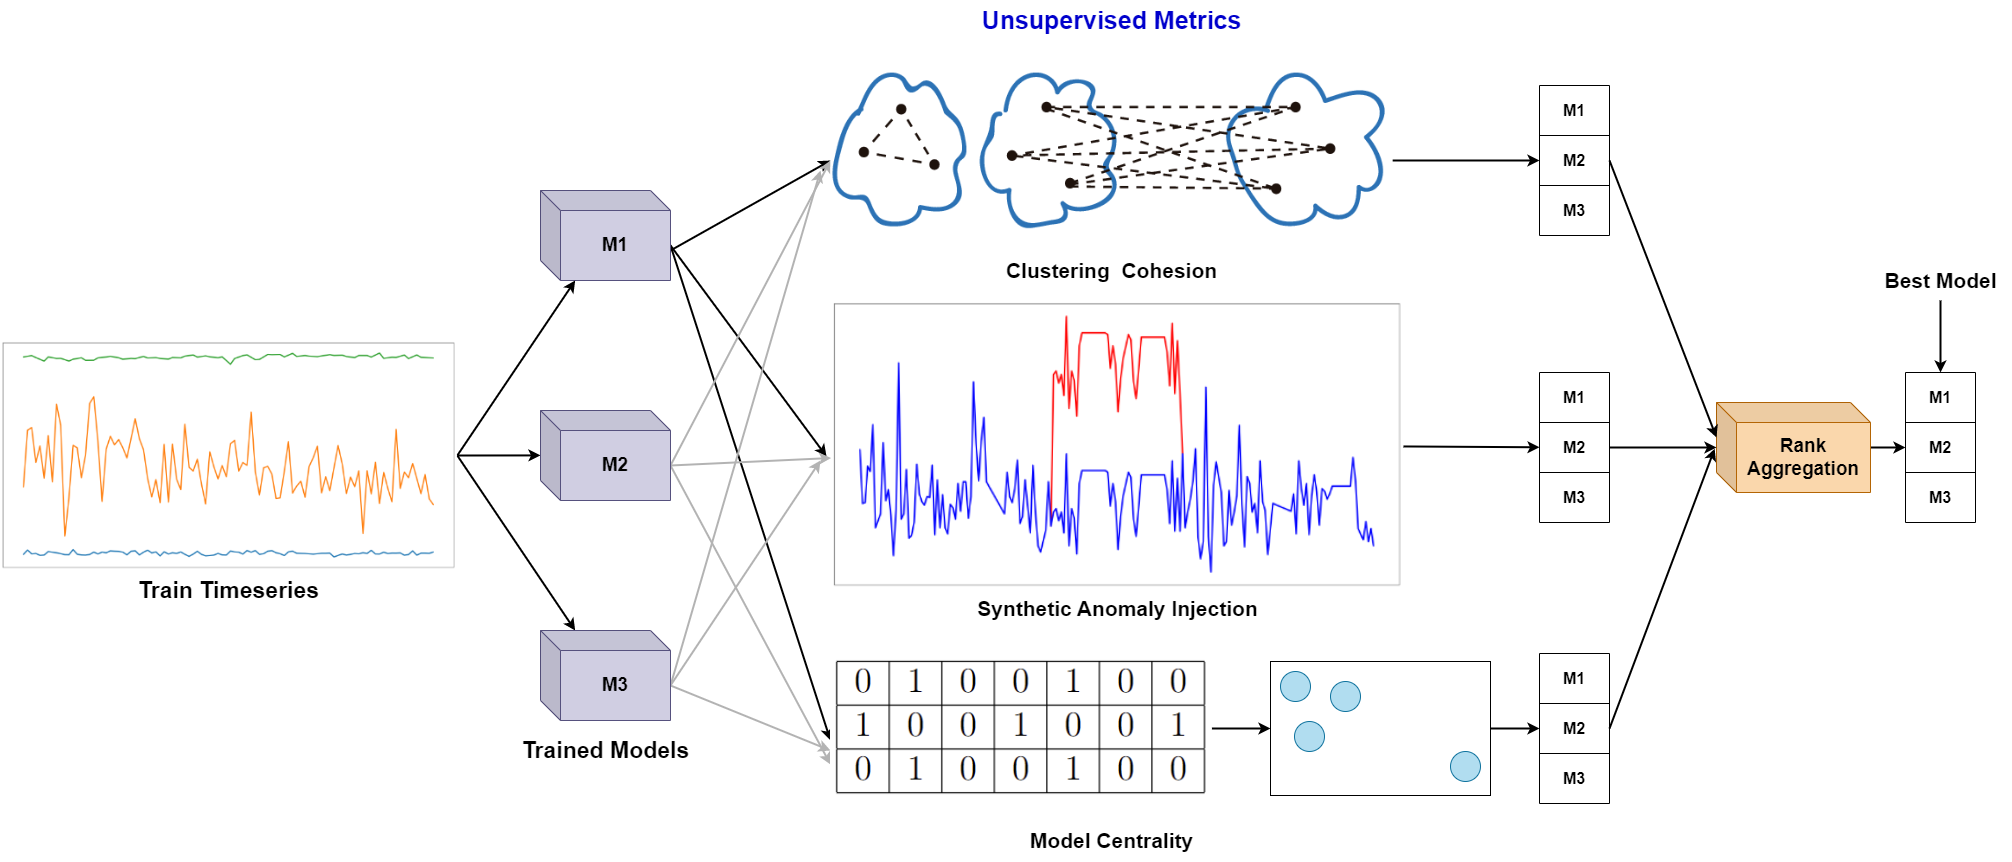
\includegraphics[width=14cm, scale=1]{images/model-selection-scheme}
	\caption{Flusso operazionale}
	\label{flow-scheme}
		
\end{figure}

\subsection{Metriche Surrogate}
Ogni metrica non supervisionata serve come misura della bontà di un modello e riduce il problema del Model Selection ad una selezione di quello con lo score piu alto. 
Sono state identificate tre classi di metriche e vengono definite non supervisionate in quanto non richiedono labels. Tuttavia, due di queste utilizzano lo F1 Score, tipicamente utilizzato per la valutazione supervisionata; per evitare confusione viene quindi utilizzato il termine "surrogato".
Di seguito viene analizzata ogni classe di metriche surrogate. 


\subsubsection{Model Centrality}
\textit{Esiste una sola ground truth, quindi i modelli vicini a questa sono anch'essi vicini tra loro ed il modello più "centrale" è il migliore.}
Metodi basati sulla centralita hanno ottenuto successi recenti nel Model Selection e nell'Anomaly Detection. 
Per adottare quest'idea si e' fatto uso di diverse tecniche che andassero a produrre dei ranking nella quale i modelli con score piu alto erano indicati come quelli piu "centrali".
Sono strate proposte 4 metodi per computare lo score di model centrality. Ognuna di queste riceve come input un set di K modelli a cui e' stato fatto training non supervisionato su un dataset di riferimento. 
\begin{itemize}
	\item \textbf{Round Robin}: dati i K modelli, ognuno di questi viene selezionato a turno e le sue labels vengono usate come ground truth per valutare le performance degli altri K-1 modelli. Infine viene prodotto un unico ranking finale andando a calcolare la media delle performance di ogni modello rispetto alle k-1 iterazioni. 
	\item \textbf{Majority Vote} e' il metodo piu semplice per generare consenso: dati K modelli e le loro labels, viene generato un nuovo set di labels finale andando a prendere, per ogni sample, la label che riceve piu voti. Questo nuovo set viene usato come ground truth per valutare i K modelli.
	\item \textbf{Sampling}: per ogni sample all'interno del dataset viene scelto in maniera casuale un modello da usare per estrarre la label per quel sample. Viene quindi prodotto un nuovo set di labels da usare come ground truth per valutare i K modelli.
	\item \textbf{Score Correlation}: questo metodo utilizza gli scores prodotti da ogni modello, dove lo score al contrario delle labels, rappresenta un valore scalare direttamente proporzionale alla probabilita che quel sample sia anomalo. Vengono infatti calcolati i ranking per ognuno di questi set di scores: Sia $Ok(i)$ il rango del sample $i$ secondo gli scores prodotti dal modello K. Viene definita la distanza dal modello $Ak$ al modello $Al$ come la distanza di Kendall, ovvero il numero di disaccordi per ogni possibile coppia. Infine viene misurata la centralita di un modello come la distanza media rispetto ai suoi M vicini, dove M e' un parametro.
\end{itemize}

Ognuna di questi metodi produce un ranking finale per cui i modelli con lo score piu alto sono quelli piu centrali. In particolare i metodi Round Robin, Majority Vote e Samplig che utilizzando un ground truth generata sul momento, utilizzando lo F1 Score per valuatare ogni modello rispetto a questa ground truth.
Questa metrica surrogata non e' perfetta, mentre funziona bene quando i modelli candidati sono tutti sufficientemente buoni da un punto di vista delle performance; nel caso siano presenti un numero relativamente alto di modelli "non buoni", questi potrebbero produrre risultati simili e formare un cluster che va di fatto a condizionare la centralita'.
Nella parte della valutazione su dataset di benchmark verranno analizzate le performance di ognuna di queste 4 metodologie.


\subsubsection{Performance on Synthetic Anomaly Injection}
\textit{Un buon modello di Anomaly Detection si comporterà bene anche su dataset con anomalie iniettate sinteticamente}. Alcuni paper hanno precedentemente esplorato l'uso dell'iniezione di anomalie sintetiche per addestrare
modelli di rilevamento delle anomalie [Carmona et al,
2021]. Attraverso questa metrica surrogata, viene estesa questa linea di ricerca
valutando sistematicamente la capacità dell'algoritmo di Model Selection dopo aver iniettato diversi tipi di anomalie. Data una serie temporale di input senza labels, viene iniettata casualmente un'anomalia di un determinato tipo. La posizione dell'anomalia iniettata viene trattata come una label pseudo-positiva, mentre il resto dei punti temporali sono trattati come labels pseudo-negative. 
Infine ogni modello viene valutato attraverso l'F1 Score rispetto alle pseudo-labels.

Invece di affidarsi a modelli generativi complessi [Wen et al., 2020], e' stato sviluppato un semplice algoritmo che inietta anomalie di diverso tipo andando prima ad analizzare il dataset ricevuto in input. I tipi di anomalie iniettate prese in considerazione sono 3 e sono visibili in figura \ref{tipi-anomalie}: 
\begin{figure}[t]
	\centering
	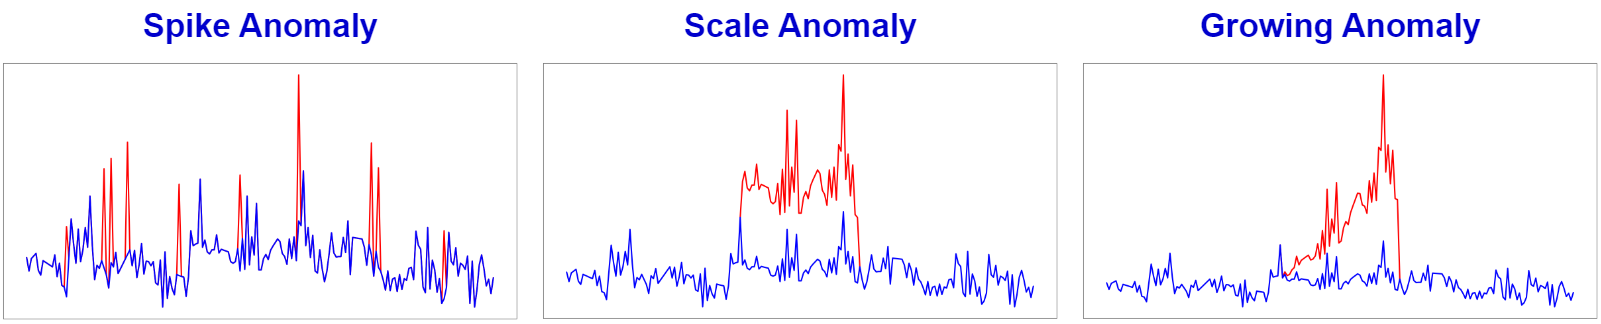
\includegraphics[width=14cm, scale=1]{images/anomalies}
	\caption{Tipologie di anomalie}
	\label{tipi-anomalie}
		
\end{figure}


\begin{enumerate}
	\item \textbf{Spike Anomaly} sono delle point anomalies in cui il valore nel punto si discosta in maniera significativa rispetto all'intorno. Lo spike ha un magnitudo governato da una distribuzione \[s \approx N(1.5, 3) \]
	\item \textbf{Scale Anomalies} e' un intervallo di punti anomali in cui il  valore medio dei punti al suo interno e' significaticamente piu grande o piu piccolo rispetto all'intorno. I dati vengono scalati \[ ts_a[i, start:end] = factor*ts[i, start:end]\] dove factor segue sempre la distribuzione \(s \approx N(1.5, 3) \)
	\item \textbf{Wander Anomalies} e' un intervallo di punti anomali in cui il valore di essi cresce o decresce linearmente nel tempo. I dati vengono modificati secondo \[ ts_a[i, start:end] = np.linspace(0, baseline, end-start) + ts[i, start:end] \] 
\end{enumerate}

Il numero di anomalie da initiettare viene calcolato sulla base del fattore di contaminazione associato ad un determinato dataset. Ad esempio, su un dataset con 10000 sample ed un fattore di contaminazione di 0.05, 500 anomalie saranno iniettate.
La posizione nella quale vengono iniettate le spike anomalies viene scelta casualmente; invece per quanto riguarda le scale e wander anomalies, vengono generati casualmente dei punti di inizio intervallo anomalo mentre la lunghezza di questi e' predisposta a mano in base alla frequenza dei sample o alla dimensione del dataset.

Attraverso uno studio di correlazione fra le feature del dataset si e' andanto a scoprire se due o piu feature devono essere considerate insieme quando si aggiunge un'anomalia in un determinato punto. In un esempio pratico, se la feature della Pressione e quella del Flow hanno una correlazione vicina a -1, quindi negativa, l'iniezione dell'anomalia prevede che una delle due feature vede il suo valore modificato verso l'alto mentre l'altro verso il basso. L'immagine \ref{feature-correlazioni} mostra un esempio di correlazioni positiva e negativa.
\begin{figure}[t]
	\centering
	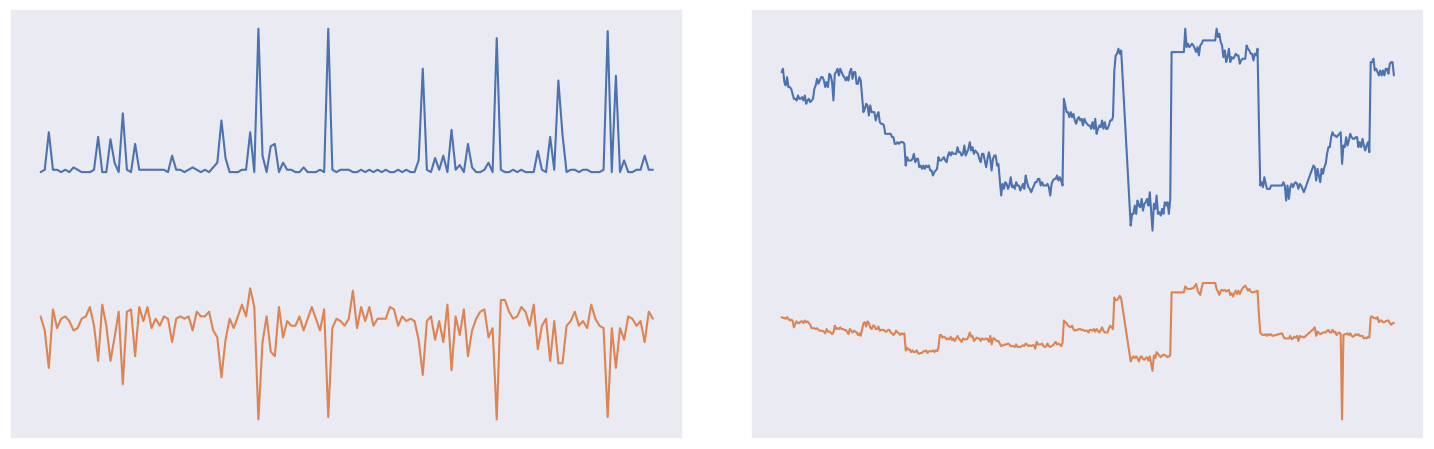
\includegraphics[width=14cm, scale=1]{images/corr}
	\caption{Correlazioni tra features}
	\label{feature-correlazioni}
		
\end{figure}

Utilizzando il coefficiente di Skew si va a vedere in che direzione portare l'anomalia: se verso il basso o verso l'alto. Feature con un right-skew avranno anomalie orientate verso l'alto, left-swek verso il basso mentre se non rientrano in nessuno dei due casi allora si generano anomalie casuali o verso il basso o verso l'alto.

Infine, calcolando l'indice di Kurt di definisce la probabilita con cui si sceglie una determinata feature per inserirvi un anomalia per ogni determinato punto. Un valore di Kurt piu alto indica una probabilita di anomalie piu alta per quella feature, questo per andare a favorire la generazione di anomalie per quelle feature che hanno una deviazione standard molto alta, al contrario di feature piu "piatte" che cambiano di rado.


Le tipologie di anomalie sintetiche possono essere iniettate in modo esclusivo, ovvero vengono generate N copie del dataset originario a cui si inseriscono una sola tipologia di anomalie sintetiche per ognuna; oppure combinandole insieme in un unico dataset. 
Ognuno di questi dataset prodotti viene poi utilizzato per effettuare la valutazione sui modelli generando quindi N rankings differenti. Le performance di ognuno di questi metodi verranno valutate successivamente.

Il flusso di lavoro di questa metrica surrogata puo essere riassunta in questi step:
\begin{enumerate}
	\item Training dei modelli sul dataset originario
	\item Creazione di dataset modificati andando ad iniettare i diversi tipi di anomalie e producendo quindi le pseudo-labels
	\item Valutazione dei modelli sui dataset modificati usando le pseudo-labels come ground truth e F1 Score come metrica di valutazione.
\end{enumerate}


Questa procedura puo essere molto efficace ma non e' esente da problemi: (1) le anomalie reali non vengono considerate e di conseguenza sono labellate come pseudo-negative. Questo potrebbe portare a score falsati nel caso i modelli andassero a riconoscere prevalentemente solo le anomalie reali, che pero' nella fase di valutazione vengono visti come sample negativi. Infine (2) le tipologie di anomalie iniettate possono risultare molto differenti da quelle che sono le reali anomali, rischiando quindi di produrre score molto alti per certi modelli ma che nella realta funzioneranno particolarmente male sul dataset originario.

\subsubsection{Clustering Cohesion}
\textit{Un buon modello riesce a trovare una buona separazione tra i punti normali ed i punti anomali}.
Nel contesto dei modelli non supervisionati, tecniche e metriche di valutazione inerenti al clustering sono molto efficaci quando non si hanno a disposizione le labels. Misure di coesione tra i cluster prodotti da un modello sono indicatori di quanto quest'ultimo sia riuscito a separare efficacemente i dati.
All'interno del task dell'Anomaly Detection, le anomalie sono punti che di discostano in maniera significativa da un comportamento normale e di conseguenza avranno valori molto diversi rispetto al resto dei punti. Immaginando i punti considerati normali con un unico cluster, ci si aspetta che questi siano ben raggruppati insieme mentre i punti anomali sono sparsi o al piu raggruppati in zone poco dense.
\begin{center}
	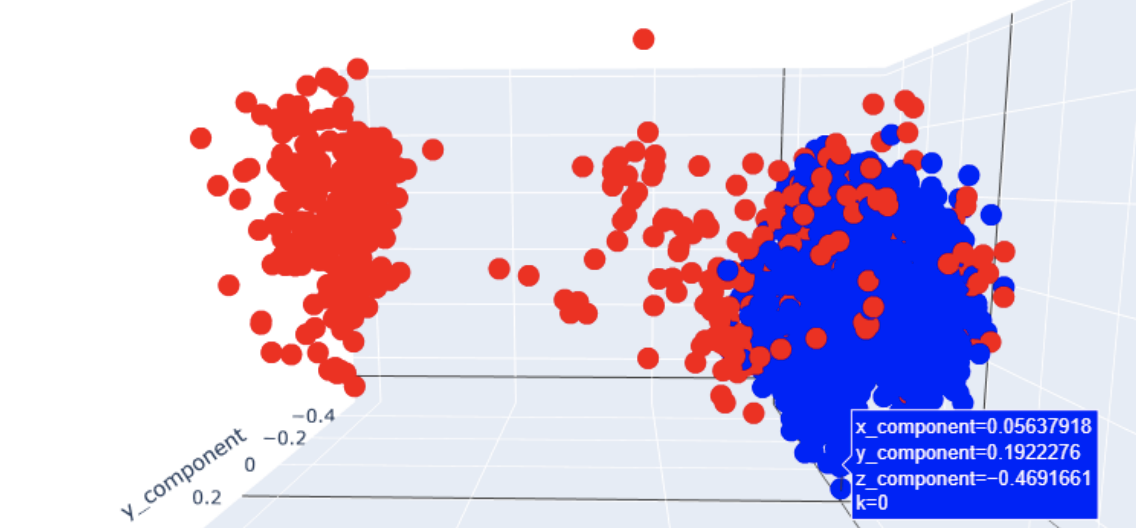
\includegraphics[width=12cm, scale=1]{images/plot-anomalies-normal}
    \captionsetup{type=figure}
	\captionof{figure}{Scatter plot dopo l'Anonaly Detection}
\end{center}
L'idea alla base di questa metrica surrogata e' quindi quella di calcolare la coesione e separazione tra il cluster di punti normali e quello di punti anomali prodotti dalle labels di un modello di Anomaly Detection. Piu alto e' questo score, piu il modello riesce a separare questi dati e quindi puo essere considerato come un buon modello.
La metrica utilizzata e' il Silouetthe Score, ma non viene calcolata subito dopo aver ottenuto le labels da un modello, sono neccessari prima alcuni passaggi di preprocessing.
Immaginiamo di avere un dataset con due feature per la quale e' possibile plottare graficamente i punti in un piano cartesiano. Idealmente i punti considerati normali formano un unico cluster denso, ma la stessa cosa non si puo dire per i punti anomali.



Questi possono essere sparsi per il piano come se fossero rumore oppure possono formare numerosi cluster di piccole dimensioni. Calcolare il silouette score assumendo solo questi due cluster il risultato potrebbe risultare falsato proprio per il fatto che i punti sparsi contribuiscono in maniera negativa allora score.
La soluzione adottata e' quella di applicare l'algoritmo di DBSCAN sui punti anomali, per formare quindi piu cluster da questi e per scartare quei punti che vengono labellati dall'algoritmo come rumore.
Prima di fare cio pero e' necessario ridurre la dimensionalita dei dati per evitare il problema del "Curse Of Dimensionality", il quale afferma che in un dataset ad alta dimensionalita', la distanza tra i singoli punti e' troppo alta per essere informativa.
Applicando quindi PCA per riddure le dimensioni a 3, rende l'applicazione di DBSCAN piu efficace. Come parametri sono stati usati $min_samples=dim * 2$ e per quanto riguarda $eps$ e' stato ricavato il valore usando l'elbow method.
Applicando quindi DBSCAN si ottengono i clster per i punti anomali.
\begin{center}
	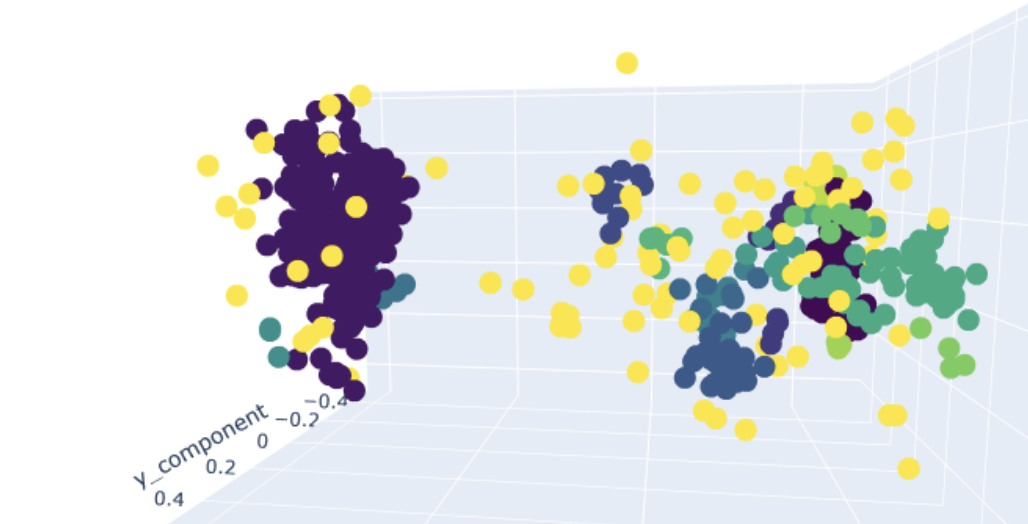
\includegraphics[width=12cm, scale=1]{images/plot-dbscan-anomalies}
    \captionsetup{type=figure}
	\captionof{figure}{Scatter plot dopo DBSCAN sulle anomalie}
\end{center}

Infine viene calcolato il silouette score su questi, tenendo anche in considerazione il cluster di punti normali originario.

Infine questa procedura viene applicata su ogni modello per andare a produrre un ranking finale.
Questa metrica surrogata puo funzionare particolarmente bene quando l'autocorrelazione di una serie temporale e' relativamente bassa e quindi i punti sono quasi indipendenti tra di loro. Le point anomalies cosi come le collective anomalies sono identificate con piu precisione rispetto alle contextual anomalies. Infatti, per definizione, i primi due tipi rappresentano punti molto distanti rispetto all'insieme totale, mentre il terzo tipo rappresenta punti distanti rispetto ad un intorno ma che potrebbero essere valutati normali rispetto ad altri intervalli, risultando quindi con piu probabilita nel cluster di punti normali.
\subsection{Rank Aggregation}
Nel capitolo \ref{chap:modelselection} e' stata fatta una panoramica su Rank Aggregation, vediamo ora quali tecniche sono state implementate. Un'analisi sulle performance di ognuno sara' svolta nelle sezioni successive.
Ognuno di questi metodi riceve in input un set di rankings, ognuno prodotto da una metrica surrogata diversa, ed in output viene generato un unico ranking finale.
Nel caso delle metriche surrogate Model Centrality e Performance on Anomaly Injection, il ranking prodotto si basa sul F1 Score; mentre per Clustering Cohesion sul Silouette Score.
\subsubsection{Kemeny-Young}
E' il metodo di Rank Aggregation ottimale in quanto ottimizza la funzione oggetto come definito nel capitolo \ref{chap:modelselection}. E' un problema NP-Hard ma la complessita temporale, dati solo 3 ranking, e' sufficientemente bassa da garantirne un utilizzo in tempo reale. Nella tabella \ref{kemeny-young}, viene proposto un esempio di Ranking Aggregation con questo metodo. Le prime tre colonne rappresentano i 3 rankings delle metriche surrogate mentre gli indici di riga corrispondono a 3 modelli.
\begin{table}
	\centering
	\caption{\label{kemeny-young}Esempio di aggregazione con Kemedy-Young.}
	\begin{tabular}{|l|l|l|l|l|} 
		\hline
		   & MC  & PAI & CC  & Final Ranking \\ 
		\hline
		M1 & 1   & 0.5 & 0.7 & 0.784         \\ 
		\hline
		M2 & 0.8 & 0.6 & 0.7 & 0.742         \\ 
		\hline
		M3 & 0.6 & 0.7 & 0.8 & 0.930         \\ 
		\hline
		M4 & 0.5 & 0.8 & 0.5 & 0.696         \\
		\hline
	\end{tabular}
\end{table}

\subsubsection{Borda}
I tre ranking prodotti dalle metriche surrogate contenenti gli score per ogni modello vengono convertiti in semplici ranking di posizione in cui il modello con lo score piu alto sara' in posizione 1. Successivamente per ognuno dei tre ranking viene assegnato un punteggio al modello in base alla posizione in cui si trova: il modello piu in basso ricevera 1 punto, il secondo piu in basso 2 punti e cosi via. Il modello in prima posizione ricevera un numero di punti uguale al numero di modelli. A questo punto vengono effettuati i calcoli per ognuna delle 3 metriche surrogate ed il punteggio finale, per ogni modello, sara' la media dei 3 valori ottenuti.

\begin{table}
	
	\centering
	\begin{tabular}{|l|l|l|l|l|l|l|l|}
		\hline
		   & MC  & PAI & CC  & B(MC) & B(PAI) & B(CC) & Final Ranking \\ \hline
		M1 & 1   & 0.5 & 0.7 & 4     & 1      & 2.5   & 2.5           \\ \hline
		M2 & 0.8 & 0.6 & 0.7 & 3     & 2      & 2.5   & 2.5           \\ \hline
		M3 & 0.6 & 0.7 & 0.8 & 2     & 3      & 4     & 3             \\ \hline
		M4 & 0.5 & 0.8 & 0.5 & 1     & 4      & 1     & 2             \\ \hline
	\end{tabular}
	\caption{\label{borda}Esempio di aggregazione con Borda.}
\end{table}


Nella tabella \ref{borda}, viene riproposto l'esempio precedente ma utilizzando Borda. Le prime 3 colonne sono gli stessi score delle metriche surrogate, invece le seconde 3 colonne rappresentano i punteggi che ogni modello ha ricevuto secondo il metodo Borda. Infine, l'ultima colonna rappresenta il punteggio medio. Lo score piu alto e' stato ottenuto dal modello M3, risultando poi primo nella classifica finale.
\subsubsection{Robust Borda}
E' una variazione del metodo Borda in cui viene scelto un parametro $k$ e per ogni ranking viene assegnato il punteggio solamente ai top-k modelli mentre i restanti vengono considerati come se fossero tutti in ultima posizione, ricevendo cosi il punteggio minimo. Questo metodo cerca di migliorare le performance del metodo Borda classico andando a penalizzare i modelli che finiscono in ultima posizione in un determinato ranking. 

\begin{table}
	
	\centering
	\begin{tabular}{|l|l|l|l|l|l|l|l|}
		\hline
		   & MC  & PAI & CC  & rB(MC) & rB(PAI) & rB(CC) & Final Ranking \\ \hline
		M1 & 1   & 0.5 & 0.7 & 4      & 1       & 2.5    & 2.5           \\ \hline
		M2 & 0.8 & 0.6 & 0.7 & 3      & 1       & 2.5    & 2.16          \\ \hline
		M3 & 0.6 & 0.7 & 0.8 & 1      & 3       & 4      & 2.66          \\ \hline
		M4 & 0.5 & 0.8 & 0.5 & 1      & 4       & 1      & 2             \\ \hline
	\end{tabular}
	\caption{\label{rborda}Esempio di aggregazione con Robust Borda.}
\end{table}

Continuando con lo stesso esempio in tabella \ref{rborda} e assumendo il parametro \(k=2\), i punteggi di Borda per Model Centrality e Performance on Anomalies Injection cambiano rispettivamente per i modelli M3 e M2 che ricevono entrambi il punteggio minimo, ovvero 1, nonostante non siano ultimi andando a penalizzare il loro score finale. M3 e' sempre quello con score piu alto ma in questo caso la differenza con M1 si e' fatta piu piccola.

\subsubsection{Score}
Questo metodo e' il piu semplice dei 3 in quanto viene semplicemente fatta una media degli score dei 3 ranking per ogni modello, per poi ordinare in ordine decrescente e quindi ottenere un ranking finale.
Utilizzando questo metodo e sempre considerando gli stessi score degli esempi precedenti, in tabella \ref{score} si puo notare come questa volta il modello migliore sia M2 e non piu M3.

\begin{table}
	
	\centering
	\begin{tabular}{|l|l|l|l|l|}
		\hline
		   & MC  & PAI & CC  & Final Ranking(avg) \\ \hline
		M1 & 1   & 0.5 & 0.7 & 0.73               \\ \hline
		M2 & 0.8 & 0.6 & 0.7 & 0.7                \\ \hline
		M3 & 0.6 & 0.7 & 0.8 & 0.7                \\ \hline
		M4 & 0.5 & 0.8 & 0.5 & 0.6                \\ \hline
	\end{tabular}
	\caption{\label{score}Esempio di aggregazione con Score.}
\end{table}



Chiaramente il processo di Ranking Aggregation aggiunge complessita e variabilita al processo di Model Selection, un'analisi sui risultati di ognuno dei metodi appena proposti e' riportata nella sezione successiva. Il generale pero, il metodo ottimale di Kemeny-Young risultera il migliore e sara' poi quello utilizzato su SKF.


\subsection{Valutazione}
Per confrontare i risultati ottenuti dalle metriche surrogate si e' deciso di adottare le misure di correlazione tra rank o tra gli score dei rankings rispetto a quelli ottenuti usando le labels. Per questi ultimi, la metrica scelta e' F1 Score.
Quindi, utilizzando l'algoritmo di Model Selection, vengono prodotti rankings contententi gli score di ogni modello per ogni metrica surrogata piu un ranking per ogni tecnica di aggregazione. Confrontare ogni singola metrica surrogata e non soltanto l'aggregazione finale permette di avere una panoramica completa delle performance di ognuno.
Questi vengono confrontato con il ranking prodotto  da una valutazione usando le labels ground-truth dei dataset di bencharmk con F1 Score.
Gli algoritmi di calcolo per il coefficiente di correlazione sono Kendall e Spearman per il rank correlation e Pearson per lo score correlation. Tutte e tre i coefficienti hanno un range compreso tra $[-1,1]$ dove un coefficiente di -1 indica una correlazione negativa, 0 nessuna correlazione mentre 1 una correlazione positiva. 
Dato che questi coefficienti hanno caratteristiche diverse e' necessario andare a trattare separatamente il calcolo:
\begin{itemize}
	\item Rank Correlation: Kendall e Spearman utilizzando dei rank di posizione per calcolare il coefficiente di correlazione. Questo vuol dire che bisogna andare a trasformare tutti i rankings con gli score in rakings di posizione in cui il modello con score piu alto avra' come posizione 1 ed i restanti a seguire.
	\item Score Correlation: Pearson invece necessita di valori continui di conseguenza per questo coefficiente non si effettua nessuna trasformazione e si usano i rankings con gli score cosi come sono prodotti dal Model Selection
\end{itemize}

 

\newpage
\section{Benchmark Results}
\subsection{Dataset}
I dataset trattati sono diversi sia per struttura ma anche per tipologia: verranno dapprima introdotti semplici dataset multidimensionali a punto per poi passare a serie temporali multivariate. 

\subsubsection{ODDS}
Outlier Detection DataSets e' una collezione di dataset per l'Outlier Detection. Questo archivio e' in continuo sviluppo dal 2016 da parte di numerosi ricercatori e comprende dataset di vari domini, dimensione, numero di features e percentuale di anomalie. 
Sono presenti sia dataset multi-dimensionali a punto che dataset nella forma di serie temporali multivariate. Da questo archivio dati verranno presi in considerazione soltato i dataset del primo tipo; in particolare, verranno trattati i seguenti dataset multi-dimensionali a punto.

La tabella \ref{odds} elenca tutti i dataset di ODDS utilizzati.

\begin{table}
	
	\centering
	\begin{tabular}{|l|l|l|l|l|}
		\hline
		\textbf{Dataset} & \textbf{\#points} & \textbf{\#dim} & \textbf{\#outliers(\%)} & \textbf{domain} \\ \hline
		annthyroid       & 7200              & 6              & 534 (7.42\%)            & Healthcare      \\ \hline
		cardio           & 1831              & 21             & 176 (9.61\%)            & Healthcare      \\ \hline
		cover            & 286048            & 10             & 2747 (0.96\%)           & Botany          \\ \hline
		donors           & 619326            & 10             & 36710 (5.93\%)          & Sociology       \\ \hline
		mammography      & 11183             & 6              & 260 (2.32\%)            & Healthcare      \\ \hline
		PageBlocks       & 5393              & 10             & 510 (9.46\%)            & Document        \\ \hline
		satimage-2       & 5803              & 36             & 71 (1.22\%)             & Astronautics    \\ \hline
		shuttle          & 49097             & 9              & 3511 (7.15\%)           & Astronautics    \\ \hline
		thyroid          & 3772              & 6              & 93 (2.47\%)             & Healthcare      \\ \hline
		vowels           & 1456              & 12             & 50 (3.43\%)             & Linguistics     \\ \hline
		Waveform         & 3443              & 21             & 100 (2.9\%)             & Physics         \\ \hline
		Wilt             & 4819              & 5              & 257 (5.33\%)            & Botany          \\ \hline
	\end{tabular}
	\caption{\label{odds}Dataset ODDS}
\end{table}

Per questi dataset si e' deciso di adottare uno train/test split costituito da 66\% per il train e 33\% per il test. I dataset di train contengono al loro interno anche una percentuale di anomalie. Potrebbe non essere la situazione ideale in quanto e' consigliato per i modelli non supervisionati di essere allenati e quindi apprendere da dati il piu puliti possibili. Ma e' la situazione piu realistica in quanto nella realta la presenza di label non e' sempre garantita.  

\subsubsection{SMD}
Server Machine Dataset e' un dataset proveniente da una compagnia Internet, consiste in serie temporali multivariate della durata di 5 settimane in cui ogni osservazione e' equamente distribuita da una frequenza di 1 minuto. SMD contiene tre gruppi di macchinari (denotati SMD-1, SMD-2 e SMD-3 rispettivamente) per un totale di 28 macchinari, ed ognuno di questi ha 38 features. Sono presenti approssimativamente 28000 time step e sono divisi in due parti della stessa lunghezza come train e test set. 
La percentuale di anomalie al suo interno si attesta intorno al 4.16 e si trovano tutte nelle ultime due settimane di dati. In questo caso, le prime tre settimane sono usate per fare il training dei modelli mentre le ultime due per la valutazione di questi.



\subsection{Modelli}
Per una valutazione piu completa si e' deciso di utilizzare un alto numero di modelli ognuno con caratteristiche e proprieta differenti. Algoritmi di Machine Learning basati sulla distanza, probabilistici o lineari; ma anche Neural Network come Auto Encoders o LSTM. La tabella \ref{admodels} e' compresiva di tutti i modelli considerati.

Gli algoritmi di machine learning considerano i sample in maniera indipendente, mentre quelli a rete neurale considerano una finestra temporale per per andare a fare sia training che prediction, risultando quindi time-aware, ovvero tengono in considerazione l'aspetto temporale dei dati. Il valore di questa finestra temporale viene passato come parametro e valorizzato manualmente.

Come definito nel capitolo \ref{chap:modelselection}, questi modelli producono in output uno score per ogni sample utilizzato per la predizione dove uno score piu alto indica una probabilita maggiore che quel modello sia anomalo. Questi score vengono trasformati in labels \(\in \{0,1\}\) andando a specificare un fattore di contaminazione, ovvero la percentuale di punti anomali. I sample che rientrano nell'insieme costituito da un numero di elementi pari alla percentuale definita prima con lo score piu alto avranno una label che indicano che sono anomali.

Ognuno di questi modelli e' stato allenato utilizzando sia i valori predefiniti per gli iper-parametri, sia variazioni di questi. 
Per ogni algoritmo sono state considerate in media 3 versioni con parametri differenti, portando il totale dei modelli a 70.
La scelta dei valori modificati agli iper-parametri e' stata fatta manualmente a priori, senza conoscere le performance del modello. Il focus della tesi si mantiene sul Model Selection, mentre un approfondimento sul tuning dei parametri puo essere lasciato a sviluppi futuri.

Il fattore di contaminazione passato ad ogni modello corrisponde esattamente alla percentuale di anomalie presenti in ogni dataset di benchmark. Questa situazione e' ottimale in quanto il numero di punti anomali trovati dai modelli coincide con il numero di anomalie reali. Ovviamente non e' possibile replicare questo anche sul dataset di SKF in quanto qualsiasi informazione sulle anomalie non e' presente. Per risolvere questo problema si utilizzera un metodo di Tresholding come introdotto nel capitolo \ref{chap:methods} che stima il fattore di contaminazione. Un fattore di contaminazione stimato male porta ovviamente a degradare le performance del Model Selection. Cosi come per la variazione degli iper-parametri, in sviluppi futuri potrebbe risultare utile un'analisi piu approfondita andando anche a testare l'algoritmo con diversi valori per il fattore di contaminazione.


\begin{table}[]
	\caption{\label{admodels}Algoritmi di Anomaly Detection}
	\centering
	\resizebox{\textwidth}{!}{%
		\begin{tabular}{|l|l|l|}
			\hline
			\textbf{Model} & \textbf{Type}     & \textbf{Algorithm}                                                  \\ \hline
			ECOD           & Probabilistic     & Outlier Detection Using Empirical Cumulative Distribution Functions \\ \hline
			COPOD          & Probabilistic     & Copula-Based Outlier Detection                                      \\ \hline
			ABOD           & Probabilistic     & Angle-Based Outlier Detection                                       \\ \hline
			SOS            & Probabilistic     & Stochastic Outlier Selection                                        \\ \hline
			KDE            & Probabilistic     & Outlier Detection with Kernel Density Functions                     \\ \hline
			Sampling       & Probabilistic     & Rapid distance-based outlier detection via sampling                 \\ \hline
			GMM            & Probabilistic     & Probabilistic Mixture Modeling for Outlier Analysis                 \\ \hline
			PCA            & Linear Model      & Principal Component Analysis                                        \\ \hline
			KPCA           & Linear Model      & Kernel Principal Component Analysis                                 \\ \hline
			MCD            & Linear Model      & Minimum Covariance Determinant                                      \\ \hline
			OCSVM          & Linear Model      & One-Class Support Vector Machines                                   \\ \hline
			LMDD           & Linear Model      & Deviation-based Outlier Detection                                   \\ \hline
   			AutoRegressive & Neural Networks   &                                                                     \\ \hline
			LOF            & Proximity-Based   & Local Outlier Factor                                                \\ \hline
			COF            & Proximity-Based   & Connectivity-Based Outlier Factor                                   \\ \hline
			CBLOF          & Proximity-Based   & Clustering-Based Local Outlier Factor                               \\ \hline
			HBOS           & Proximity-Based   & Histogram-based Outlier Score                                       \\ \hline
			kNN            & Proximity-Based   & k Nearest Neighbors                                                 \\ \hline
			SOD            & Proximity-Based   & Subspace Outlier Detection                                          \\ \hline
			ROD            & Proximity-Based   & Rotation-based Outlier Detection                                    \\ \hline
			IForest        & Outlier Ensembles & Isolation Forest                                                    \\ \hline
			INNE           & Outlier Ensembles & Isolation-based Anomaly Detection Using Nearest-Neighbor Ensembles  \\ \hline
			FB             & Outlier Ensembles & Feature Bagging                                                     \\ \hline
			AutoEncoder    & Neural Networks   & Fully connected AutoEncoder                                         \\ \hline
			VAE            & Neural Networks   & Variational AutoEncoder                                             \\ \hline
			DeepSVDD       & Neural Networks   & Deep One-Class Classification                                       \\ \hline
			ALAD           & Neural Networks   & Adversarially learned anomaly detection                             \\ \hline
			LUNAR          & Graph-based       & Unifying Local Outlier Detection Methods via Graph Neural Networks  \\ \hline
			DeepLog        & Neural Networks   &                                                                     \\ \hline
			Telemanom      & Neural Networks   &                                                                     \\ \hline
			LSTM           & Neural Networks   &                                                                     \\ \hline
		\end{tabular}%
	}
\end{table}







\subsection{Risultati}
I risultati saranno mostrati come segue: inizialmente verranno mostrati i coefficienti di correlazione per ogni singola metrica surrogata ed ognuno dei rispettivi metodi su un subset dei dataset per poi passare ad un analisi delle performance calcolate come media rispetto a tutti i dataset.

I risultati delle diverse tecniche di Rank Aggregation saranno presentati allo stesso modo: prima su un sottoinsieme dei dataset e infine come media rispetto a tutti.

Infine viene presentata un'analisi sui rank dei modelli dei rankings prodotti dalle metriche surrogate paragonati ai rank del ranking prodotto in maniera supervisionata con le label.
\subsubsection{Model Centrality}
Questa metrica surrogata si basa sul concetto di Model Centrality andando a favorire quei modelli che producono output comparabili alla maggior parte degli altri modelli. Delle quattro tecniche proposte, Round Robin e' quella che generalemente si comporta meglio. In tabella \ref{mc-results} possiamo vedere come gli indici di correlazione favoriscano questa tecnica.
Mahority Vote e Sampling seguono con punteggi molto simili, sia per le performance medie che per la standard deviation. Il metodo Score fatica a trovare correlazione con il ranking supervisionato. 
Generalmente pero', la metrica funziona discretamente bene tranne qualche dataset specifico come Machine-3-10.  Nelle immagini \ref{model-centrality-plot-bad} e \ref{model-centrality-plot-good} sono mostrati dei scatter plot di dove ogni modello si posiziona in uno spazio bidimensionale. La posizione viene calcolata riducendo a due dimensioni l'output delle predizioni di ogni modello.  Nella figura della Machine-3-10 possiamo notare come i punti sono sparsi lungo tutto il piano rendendo difficile alla metrica surrogata riuscire a trovare una definizione per modello centrale.
Per Machine-1-4, invece, le performance di correlazione sono migliori e possiamo anche notare come la maggior parte dei punti risieda nel cluster formatosi sulla sinistra. Questo permette di spostare la centralita di un modello verso quella zona ed e' anche altamente probabile che il miglior modello si trovi li, migliorando di conseguenza la correlazione tra il ranking di Model Centrality ed il ranking supervisionato.
Come si vedra piu avanti, questa metrica e' la piu stabile delle tre, ovvero che le performance variano relativamente meno rispetto ad ogni dataset. Motivo di cio e che questa metrica non lavora direttamente sui dati del dataset ma sugli output dei modelli ed e' quindi suscettibile alla lista di modelli che si passa in input al Model Selection. Se non si ha conoscenza su quali modelli potrebbero funzionare meglio e' dunque consigliato utilizzare un numero di modelli che abbiano caratteristiche diverse sufficientemente alto in modo da non rischiare di condizionare la centralita orientandola verso quei modelli meno performanti.


\begin{figure}[]
	\centering
	\begin{minipage}[b]{0.45\textwidth}
		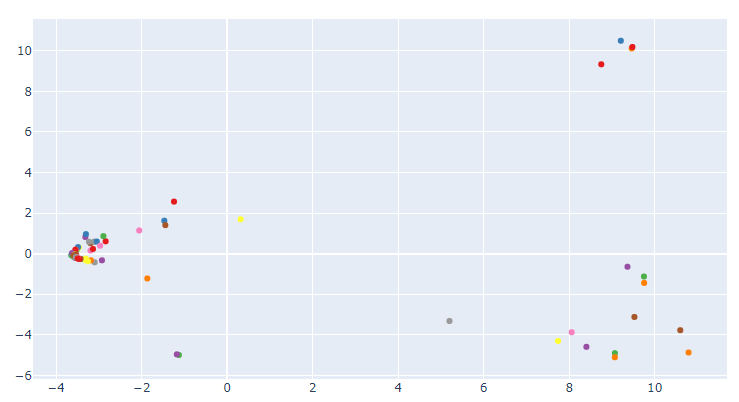
\includegraphics[width=\textwidth]{images/model_centrality_good2-8_2}
		\caption{Machine-1-4}
		\label{model-centrality-plot-good}
	\end{minipage}
	\begin{minipage}[b]{0.45\textwidth}
		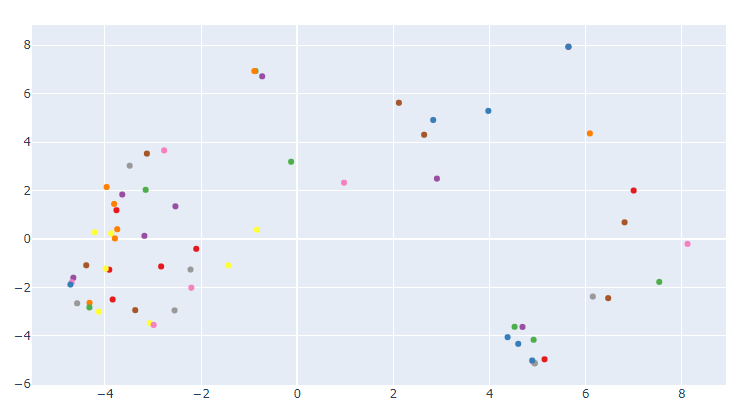
\includegraphics[width=\textwidth]{images/model_centrality_bad3-10_2}
		\caption{Machine-3-10}
		\label{model-centrality-plot-bad}
	\end{minipage}
\end{figure}

\begin{table}[]
	\caption{\label{mc-results}Risultati di correlatrazione per Model Centrality}
	\resizebox{\linewidth}{!}{%
		\begin{tabular}{|l||l|l|l|l||l|l|l|l||l|l|l|l|} 
			\hline
			Dataset           & \multicolumn{4}{c||}{SCORE CORRELATION} & \multicolumn{8}{c|}{RANK CORRELATION}                            \\ 
			\hline
			\multirow{2}{*}{} & \multicolumn{4}{c||}{PEARSON}           & \multicolumn{4}{c||}{KENDALL}  & \multicolumn{4}{c|}{SPEARMAN}   \\ 
			\cline{2-13}
			                & mv     & rr    & samp  & score  & mv    & rr    & samp  & score & mv    & rr           & samp   & score \\ 
			\hline
			2\_annthyroid   & 0.823  & 0.837 & 0.836 & 0.773  & 0.584 & 0.581 & 0.605 & 0.584 & 0.739 & 0.735        & 0.753  & 0.671 \\ 
			\hline
			6\_cardio       & 0.807  & 0.787 & 0.787 & 0.654  & 0.612 & 0.563 & 0.564 & 0.565 & 0.746 & 0.715        & 0.718  & 0.626 \\ 
			\hline
			11\_donors      & 0.514  & 0.529 & 0.526 & 0.423  & 0.541 & 0.511 & 0.529 & 0.475 & 0.665 & 0.650        & 0.670  & 0.559 \\ 
			\hline
			20\_letter      & 0.559  & 0.631 & 0.763 & 0.669  & 0.473 & 0.499 & 0.692 & 0.536 & 0.565 & 0.608        & 0.840  & 0.642 \\ 
			\hline
			23\_mammography & 0.795  & 0.829 & 0.801 & 0.607  & 0.694 & 0.722 & 0.649 & 0.439 & 0.834 & 0.821        & 0.809  & 0.561 \\ 
			\hline
			27\_PageBlocks  & 0.917  & 0.911 & 0.909 & 0.832  & 0.698 & 0.677 & 0.646 & 0.550 & 0.812 & 0.849        & 0.818  & 0.717 \\ 
			\hline
			31\_satimage-2  & 0.759  & 0.855 & 0.644 & 0.553  & 0.641 & 0.865 & 0.514 & 0.440 & 0.793 & 0.970        & 0.581  & 0.462 \\ 
			\hline
			32\_shuttle     & 0.489  & 0.846 & 0.827 & 0.661  & 0.446 & 0.774 & 0.770 & 0.565 & 0.456 & 0.894        & 0.890  & 0.728 \\ 
			\hline
			38\_thyroid     & 0.719  & 0.761 & 0.701 & 0.709  & 0.538 & 0.563 & 0.508 & 0.546 & 0.667 & 0.700        & 0.632  & 0.683 \\ 
			\hline
			40\_vowels      & 0.735  & 0.760 & 0.670 & 0.612  & 0.637 & 0.642 & 0.573 & 0.463 & 0.779 & 0.806        & 0.721  & 0.582 \\ 
			\hline
			41\_Waveform    & 0.428  & 0.464 & 0.440 & 0.481  & 0.466 & 0.582 & 0.569 & 0.423 & 0.572 & 0.709        & 0.647  & 0.541 \\ 
			\hline
			machine-1-1     & 0.561  & 0.582 & 0.641 & 0.556  & 0.458 & 0.458 & 0.499 & 0.468 & 0.558 & 0.572        & 0.607  & 0.595 \\ 
			\hline
			machine-1-2     & 0.842  & 0.877 & 0.866 & 0.771  & 0.633 & 0.732 & 0.723 & 0.570 & 0.834 & 0.839        & 0.836  & 0.738 \\ 
			\hline
			machine-1-3     & 0.949  & 0.836 & 0.828 & 0.480  & 0.855 & 0.633 & 0.645 & 0.437 & 0.934 & 0.841        & 0.826  & 0.428 \\ 
			\hline
			machine-1-4     & 0.966  & 0.949 & 0.917 & 0.576  & 0.835 & 0.706 & 0.711 & 0.412 & 0.927 & 0.842        & 0.840  & 0.553 \\ 
			\hline
			machine-1-5     & 0.441  & 0.494 & 0.465 & 0.353  & 0.458 & 0.477 & 0.456 & 0.432 & 0.587 & 0.514        & 0.584  & 0.419 \\ 
			\hline
			machine-1-6     & 0.588  & 0.551 & 0.576 & 0.585  & 0.550 & 0.527 & 0.528 & 0.521 & 0.621 & 0.582        & 0.578  & 0.601 \\ 
			\hline
			machine-1-7     & 0.630  & 0.596 & 0.626 & 0.597  & 0.546 & 0.491 & 0.543 & 0.467 & 0.693 & 0.636        & 0.680  & 0.593 \\ 
			\hline
			machine-1-8     & 0.594  & 0.563 & 0.553 & 0.628  & 0.494 & 0.421 & 0.492 & 0.406 & 0.590 & 0.433        & 0.514  & 0.553 \\ 
			\hline
			machine-2-1     & 0.791  & 0.838 & 0.847 & 0.566  & 0.561 & 0.595 & 0.563 & 0.465 & 0.653 & 0.687        & 0.690  & 0.535 \\ 
			\hline
			machine-2-2     & 0.822  & 0.824 & 0.827 & 0.683  & 0.608 & 0.594 & 0.565 & 0.503 & 0.794 & 0.770        & 0.739  & 0.601 \\ 
			\hline
			machine-2-3     & 0.825  & 0.827 & 0.834 & 0.606  & 0.648 & 0.610 & 0.638 & 0.444 & 0.819 & 0.771        & 0.798  & 0.546 \\ 
			\hline
			machine-2-4     & 0.307  & 0.309 & 0.285 & 0.192  & 0.357 & 0.348 & 0.301 & 0.389 & 0.411 & 0.369        & 0.310  & 0.317 \\ 
			\hline
			machine-2-5     & 0.044  & 0.133 & 0.126 & 0.136  & 0.332 & 0.379 & 0.351 & 0.383 & 0.380 & 0.356        & 0.326  & 0.325 \\ 
			\hline
			machine-2-6     & 0.896  & 0.872 & 0.893 & 0.568  & 0.703 & 0.648 & 0.679 & 0.511 & 0.816 & 0.823        & 0.801  & 0.594 \\ 
			\hline
			machine-2-7     & 0.882  & 0.885 & 0.839 & 0.820  & 0.683 & 0.718 & 0.662 & 0.648 & 0.823 & 0.848        & 0.806  & 0.806 \\ 
			\hline
			machine-2-8     & 0.991  & 0.989 & 0.983 & 0.803  & 0.861 & 0.876 & 0.847 & 0.532 & 0.961 & 0.966        & 0.950  & 0.627 \\ 
			\hline
			machine-2-9     & 0.627  & 0.649 & 0.664 & 0.420  & 0.492 & 0.472 & 0.480 & 0.414 & 0.597 & 0.569        & 0.571  & 0.409 \\ 
			\hline
			machine-3-1     & 0.458  & 0.467 & 0.532 & 0.485  & 0.431 & 0.444 & 0.453 & 0.381 & 0.483 & 0.504        & 0.591  & 0.427 \\ 
			\hline
			machine-3-2     & 0.613  & 0.646 & 0.670 & 0.727  & 0.595 & 0.595 & 0.627 & 0.638 & 0.753 & 0.761        & 0.785  & 0.814 \\ 
			\hline
			machine-3-3     & 0.345  & 0.379 & 0.365 & 0.388  & 0.420 & 0.384 & 0.364 & 0.468 & 0.475 & 0.451        & 0.434  & 0.454 \\ 
			\hline
			machine-3-4     & 0.158  & 0.168 & 0.224 & -0.036 & 0.271 & 0.241 & 0.293 & 0.095 & 0.331 & 0.281        & 0.334  & 0.154 \\ 
			\hline
			machine-3-5     & 0.857  & 0.871 & 0.864 & 0.521  & 0.699 & 0.774 & 0.759 & 0.470 & 0.817 & 0.880        & 0.870  & 0.523 \\ 
			\hline
			machine-3-6     & 0.338  & 0.311 & 0.292 & 0.069  & 0.393 & 0.305 & 0.391 & 0.365 & 0.463 & 0.379        & 0.351  & 0.312 \\ 
			\hline
			machine-3-7     & 0.308  & 0.361 & 0.321 & 0.299  & 0.469 & 0.447 & 0.452 & 0.365 & 0.493 & 0.464        & 0.474  & 0.443 \\ 
			\hline
			machine-3-8     & 0.648  & 0.651 & 0.700 & 0.471  & 0.579 & 0.547 & 0.590 & 0.412 & 0.696 & 0.682        & 0.727  & 0.570 \\ 
			\hline
			machine-3-9     & 0.580  & 0.477 & 0.496 & 0.431  & 0.665 & 0.589 & 0.588 & 0.463 & 0.833 & 0.710        & 0.719  & 0.595 \\ 
			\hline
			machine-3-10    & -0.009 & 0.015 & 0.116 & 0.010  & 0.269 & 0.288 & 0.300 & 0.210 & 0.348 & 0.322        & 0.324  & 0.272 \\ 
			\hline
			machine-3-11    & 0.837  & 0.626 & 0.560 & 0.372  & 0.640 & 0.465 & 0.332 & 0.348 & 0.813 & 0.470        & 0.401  & 0.315 \\ 
			\hline
			AVG             & 0.627  & 0.640 & 0.636 & 0.514  & 0.560 & 0.558 & 0.550 & 0.457 & 0.670 & 0.661        & 0.655  & 0.536 \\ 
			\hline
			STD             & 0.25   & 0.24  & 0.229 & 0.214  & 0.142 & 0.149 & 0.135 & 0.102 & 0.169 & 0.186        & 0.177  & 0.146 \\
			\hline
		\end{tabular}
	}
\end{table}

\newpage
\subsubsection{Performance on Synthethic Anomaly Injection}
Passando alla metrica surrogata usante le pseudo-label dopo l'iniezione di anomalie, possiamo notare in tabella \ref{pai-results} come generamente le performance siano inferiori rispetto alla tecnica del Model Centrality. I motivi di cio possono ricondursi agli aspetti negativi introdotti precedentemente che riguardano questo approccio: 
\begin{enumerate}
	\item come le anomalie vengono generate
	\item le anomalie reali vengano ignorate
\end{enumerate}
Il primo punto non e' banale, avere una conoscenza forte dal dataset di riferimento permette di creare anomalie che possano risultare realistiche ma spesso la cio non e' possibile. Attraverso metodi statistici si possono estrarre informazioni riguardanti l'andamento e l'evoluzione dei dati ma spesso le anomalie non seguono un pattern preciso rendendo quindi la generazione di queste un problema non triviale. 
Vediamo ora alcuni esempi di come le performance variano in base al dataset ed al tipo di anomalia iniettata. Le perfoamance dell'anomia Spike sul dataset Shuttle sono buone e a conferma di cio si puo vedere in figura \ref{shuttle-inj} come le anomalie prevalenti siano proprio di tipo spike.
Al contrario, Machine-3-5 ha performance basse per quanto riguarda wander, spike e mix, ma ottiene un punteggio di 0.84 su scale. La figura \ref{machine-3-5-inj} mostra come i punti anomali abbiamo intervalli con valori scalati verso l'alto. Infine, Machine-28 e' quello con le performance Mix piu alte, a riprova del fatto che nell'immagine \ref{machine-2-8-inj} si possono notare sia spike, sia intervalli anomali e sia valori crescenti nel tempo.
Il secondo punto puo inpattare negativemente i risultati in quanto e' possibile che il modello vada a labellare le anomalie reali come positive, nonostante abbiamo delle pseudo-label negative. Una soluzione a questo problema potrebbe essere quello di ricercare una finestra temporale del dataset che sia il piu pulita possibile dalla anomalie per poi andare ad effettuare le anomaly injection.
Anche in questo caso ci troviamo di fronte a tre metodi con performance simili con un quarto, in questo caso wander, generalmente meno performante.
\begin{figure}[htp]% [H] is so declass\'e!
	\centering
	\begin{minipage}{0.5\textwidth}
		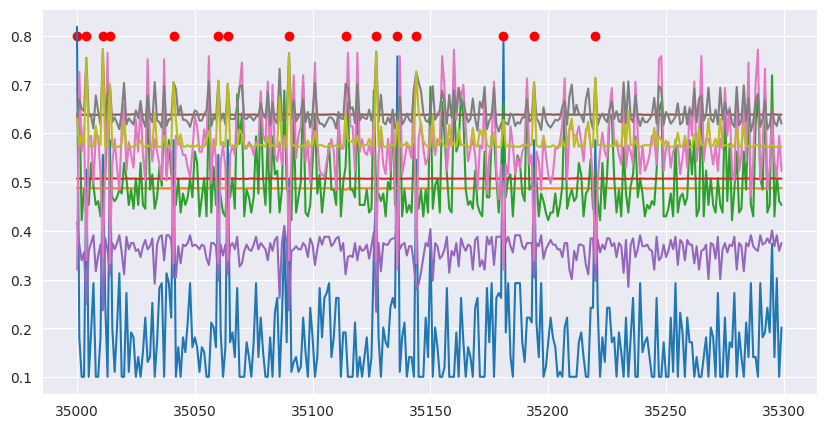
\includegraphics[width=\textwidth]{images/shuttle_good_inj_spike.png}
		\caption{Shuttle}
		\label{shuttle-inj}
	\end{minipage}\hfill
	\begin{minipage}{0.5\textwidth}
		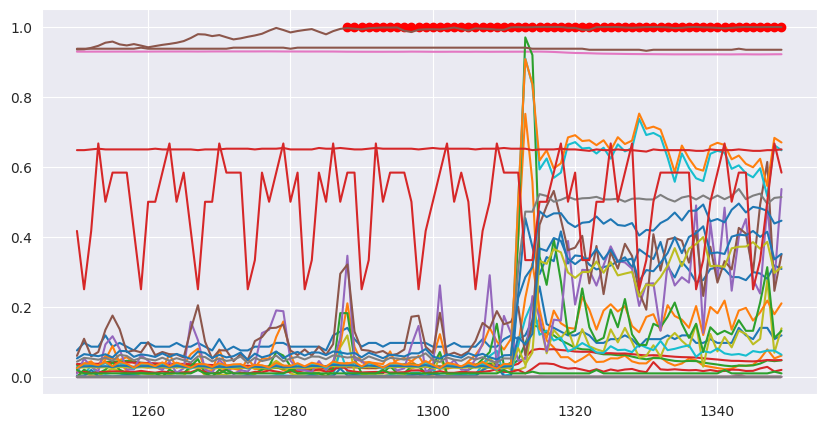
\includegraphics[width=\textwidth]{images/machine-3-5_bad_inj_good_scale.png}
		\caption{Machine-3-5}
		\label{machine-3-5-inj}
	\end{minipage}\par
	\vskip\floatsep% normal separation between figures
	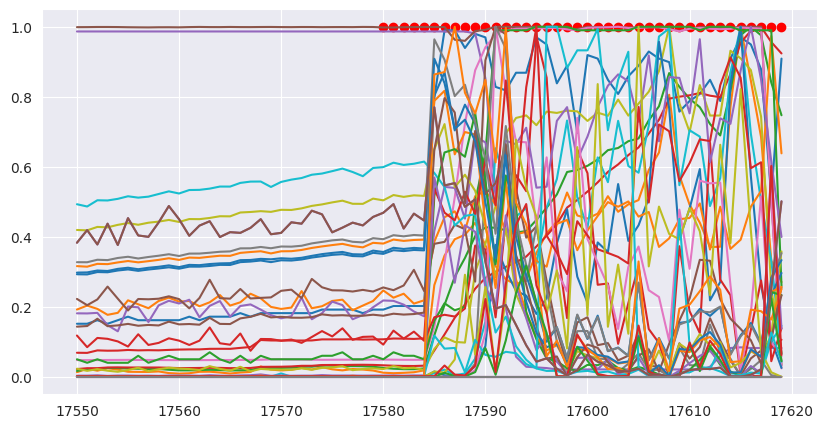
\includegraphics[width=0.5\textwidth]{images/machine-2-8_good_inj_mix.png}
	\caption{Machine-2-8}
	\label{machine-2-8-inj}
\end{figure}

\begin{table}[]
	\caption{\label{pai-results}Risultati di correlazione per Performance on Anomaly Injection}
	\resizebox{\linewidth}{!}{%
		\begin{tabular}{|l||l|l|l|l||l|l|l|l||l|l|l|l|} 
			\hline
			Dataset           & \multicolumn{4}{c||}{SCORE CORRELATION} & \multicolumn{8}{c|}{RANK CORRELATION}                            \\ 
			\hline
			\multirow{2}{*}{} & \multicolumn{4}{c||}{PEARSON}           & \multicolumn{4}{c||}{KENDALL}  & \multicolumn{4}{c|}{SPEARMAN}   \\ 
			\cline{2-13}
			                & wander & spike & scale & mix   & wander & spike & scale & mix   & wander & spike        & scale & mix   \\ 
			\hline
			2\_annthyroid   & 0.111  & 0.272 & 0.331 & 0.196 & 0.267  & 0.440 & 0.465 & 0.408 & 0.281  & 0.487        & 0.414 & 0.457 \\ 
			\hline
			6\_cardio       & 0.269  & 0.575 & 0.554 & 0.381 & 0.129  & 0.337 & 0.431 & 0.356 & 0.176  & 0.406        & 0.416 & 0.396 \\ 
			\hline
			11\_donors      & 0.331  & 0.391 & 0.316 & 0.303 & 0.472  & 0.422 & 0.442 & 0.443 & 0.491  & 0.550        & 0.575 & 0.573 \\ 
			\hline
			20\_letter      & 0.457  & 0.577 & 0.811 & 0.560 & 0.489  & 0.607 & 0.718 & 0.527 & 0.563  & 0.742        & 0.805 & 0.597 \\ 
			\hline
			23\_mammography & 0.378  & 0.401 & 0.396 & 0.494 & 0.423  & 0.562 & 0.486 & 0.535 & 0.530  & 0.671        & 0.591 & 0.597 \\ 
			\hline
			27\_PageBlocks  & 0.357  & 0.340 & 0.430 & 0.368 & 0.384  & 0.374 & 0.451 & 0.365 & 0.473  & 0.477        & 0.469 & 0.461 \\ 
			\hline
			31\_satimage-2  & 0.092  & 0.090 & 0.110 & 0.231 & 0.310  & 0.228 & 0.304 & 0.309 & 0.393  & 0.330        & 0.314 & 0.303 \\ 
			\hline
			32\_shuttle     & 0.308  & 0.333 & 0.330 & 0.355 & 0.319  & 0.303 & 0.360 & 0.344 & 0.408  & 0.368        & 0.436 & 0.414 \\ 
			\hline
			38\_thyroid     & 0.093  & 0.164 & 0.159 & 0.117 & 0.362  & 0.390 & 0.474 & 0.362 & 0.398  & 0.354        & 0.459 & 0.384 \\ 
			\hline
			40\_vowels      & 0.470  & 0.667 & 0.581 & 0.712 & 0.429  & 0.611 & 0.564 & 0.607 & 0.527  & 0.761        & 0.623 & 0.759 \\ 
			\hline
			41\_Waveform    & 0.810  & 0.775 & 0.679 & 0.764 & 0.627  & 0.571 & 0.580 & 0.639 & 0.783  & 0.737        & 0.721 & 0.823 \\ 
			\hline
			machine-1-1     & 0.379  & 0.490 & 0.597 & 0.583 & 0.425  & 0.407 & 0.697 & 0.535 & 0.557  & 0.584        & 0.835 & 0.634 \\ 
			\hline
			machine-1-2     & 0.339  & 0.373 & 0.393 & 0.364 & 0.399  & 0.316 & 0.345 & 0.351 & 0.457  & 0.354        & 0.417 & 0.368 \\ 
			\hline
			machine-1-3     & 0.117  & 0.487 & 0.335 & 0.368 & 0.334  & 0.561 & 0.325 & 0.469 & 0.210  & 0.682        & 0.180 & 0.566 \\ 
			\hline
			machine-1-4     & 0.170  & 0.206 & 0.347 & 0.193 & 0.354  & 0.444 & 0.131 & 0.309 & 0.229  & 0.489        & 0.238 & 0.313 \\ 
			\hline
			machine-1-5     & 0.108  & 0.468 & 0.209 & 0.417 & 0.316  & 0.468 & 0.383 & 0.473 & 0.360  & 0.545        & 0.325 & 0.415 \\ 
			\hline
			machine-1-6     & 0.423  & 0.566 & 0.471 & 0.441 & 0.351  & 0.449 & 0.473 & 0.405 & 0.470  & 0.575        & 0.562 & 0.494 \\ 
			\hline
			machine-1-7     & 0.301  & 0.436 & 0.351 & 0.318 & 0.329  & 0.541 & 0.432 & 0.389 & 0.397  & 0.615        & 0.440 & 0.328 \\ 
			\hline
			machine-1-8     & 0.342  & 0.472 & 0.538 & 0.357 & 0.426  & 0.429 & 0.478 & 0.368 & 0.454  & 0.447        & 0.596 & 0.350 \\ 
			\hline
			machine-2-1     & 0.516  & 0.547 & 0.497 & 0.469 & 0.502  & 0.515 & 0.479 & 0.397 & 0.576  & 0.560        & 0.446 & 0.410 \\ 
			\hline
			machine-2-2     & 0.500  & 0.464 & 0.462 & 0.516 & 0.459  & 0.403 & 0.455 & 0.476 & 0.588  & 0.523        & 0.554 & 0.591 \\ 
			\hline
			machine-2-3     & 0.555  & 0.471 & 0.470 & 0.550 & 0.540  & 0.479 & 0.428 & 0.567 & 0.647  & 0.556        & 0.540 & 0.714 \\ 
			\hline
			machine-2-4     & 0.201  & 0.422 & 0.540 & 0.522 & 0.243  & 0.425 & 0.439 & 0.517 & 0.291  & 0.443        & 0.582 & 0.584 \\ 
			\hline
			machine-2-5     & 0.459  & 0.463 & 0.401 & 0.451 & 0.498  & 0.545 & 0.558 & 0.638 & 0.579  & 0.632        & 0.712 & 0.781 \\ 
			\hline
			machine-2-6     & 0.156  & 0.438 & 0.132 & 0.404 & 0.222  & 0.462 & 0.270 & 0.492 & 0.228  & 0.569        & 0.267 & 0.596 \\ 
			\hline
			machine-2-7     & 0.391  & 0.343 & 0.450 & 0.360 & 0.476  & 0.433 & 0.468 & 0.307 & 0.495  & 0.414        & 0.560 & 0.382 \\ 
			\hline
			machine-2-8     & 0.776  & 0.330 & 0.042 & 0.771 & 0.500  & 0.345 & 0.094 & 0.510 & 0.598  & 0.423        & 0.052 & 0.575 \\ 
			\hline
			machine-2-9     & 0.463  & 0.361 & 0.329 & 0.322 & 0.512  & 0.464 & 0.366 & 0.404 & 0.577  & 0.574        & 0.429 & 0.491 \\ 
			\hline
			machine-3-1     & 0.348  & 0.366 & 0.721 & 0.411 & 0.571  & 0.507 & 0.667 & 0.520 & 0.614  & 0.566        & 0.813 & 0.580 \\ 
			\hline
			machine-3-2     & 0.443  & 0.401 & 0.374 & 0.318 & 0.474  & 0.493 & 0.402 & 0.356 & 0.453  & 0.483        & 0.455 & 0.397 \\ 
			\hline
			machine-3-3     & 0.458  & 0.336 & 0.404 & 0.347 & 0.508  & 0.336 & 0.547 & 0.467 & 0.557  & 0.432        & 0.619 & 0.457 \\ 
			\hline
			machine-3-4     & 0.351  & 0.363 & 0.408 & 0.360 & 0.442  & 0.378 & 0.415 & 0.409 & 0.445  & 0.477        & 0.542 & 0.520 \\ 
			\hline
			machine-3-5     & 0.077  & 0.188 & 0.841 & 0.036 & 0.117  & 0.255 & 0.771 & 0.035 & 0.121  & 0.240        & 0.823 & 0.056 \\ 
			\hline
			machine-3-6     & 0.513  & 0.445 & 0.359 & 0.516 & 0.450  & 0.421 & 0.338 & 0.460 & 0.576  & 0.537        & 0.314 & 0.462 \\ 
			\hline
			machine-3-7     & 0.470  & 0.486 & 0.484 & 0.406 & 0.487  & 0.551 & 0.398 & 0.493 & 0.592  & 0.702        & 0.499 & 0.484 \\ 
			\hline
			machine-3-8     & 0.371  & 0.355 & 0.202 & 0.357 & 0.464  & 0.484 & 0.271 & 0.439 & 0.432  & 0.588        & 0.350 & 0.540 \\ 
			\hline
			machine-3-9     & 0.339  & 0.310 & 0.447 & 0.378 & 0.382  & 0.387 & 0.591 & 0.472 & 0.383  & 0.484        & 0.658 & 0.463 \\ 
			\hline
			machine-3-10    & 0.344  & 0.465 & 0.398 & 0.379 & 0.428  & 0.530 & 0.541 & 0.516 & 0.486  & 0.623        & 0.613 & 0.555 \\ 
			\hline
			machine-3-11    & 0.516  & 0.663 & 0.394 & 0.693 & 0.496  & 0.504 & 0.395 & 0.551 & 0.503  & 0.607        & 0.461 & 0.693 \\ 
			\hline
			AVG             & 0.362  & 0.418 & 0.418 & 0.413 & 0.408  & 0.446 & 0.447 & 0.442 & 0.459  & 0.528        & 0.505 & 0.502 \\ 
			\hline
			STD             & 0.169  & 0.136 & 0.172 & 0.157 & 0.11   & 0.092 & 0.139 & 0.11  & 0.141  & 0.119        & 0.176 & 0.147 \\
			\hline
		\end{tabular}
	}
\end{table}

\newpage
\subsubsection{Clustering Cohesion}
Questa metrica surrogata invece va a favorire soluzioni cui le anomalie sono ben separate dai dati normali, infatti le performance variano di molto per ogni dataset preso in considerazione con un AVG score piu basso rispetto alle altre due metriche (tabella \ref{cc-results}).


\begin{table}[]
	\caption{\label{cc-results}Risultati di correlazione per Clustering Cohesion}
	\resizebox{\columnwidth}{!}{%
		\begin{tabular}{|l|l|l|l|}
			\hline
			Dataset         & \multicolumn{1}{c|}{SCORE CORRELATION} & \multicolumn{2}{c|}{RANK CORRELATION}                         \\  \hline
			                & \multicolumn{1}{c|}{PEARSON} & \multicolumn{1}{c|}{KENDALL} & \multicolumn{1}{c|}{SPEARMAN} \\ \hline
			2\_annthyroid   & 0.821                        & 0.432                        & 0.557                         \\ \hline
			6\_cardio       & 0.409                        & 0.375                        & 0.436                         \\ \hline
			11\_donors      & 0.096                        & 0.111                        & -0.049                        \\ \hline
			20\_letter      & -0.034                       & 0.061                        & -0.049                        \\ \hline
			23\_mammography & 0.368                        & 0.369                        & 0.469                         \\ \hline
			27\_PageBlocks  & 0.837                        & 0.496                        & 0.487                         \\ \hline
			31\_satimage-2  & 0.467                        & 0.389                        & 0.355                         \\ \hline
			32\_shuttle     & 0.830                        & 0.706                        & 0.832                         \\ \hline
			38\_thyroid     & 0.606                        & 0.483                        & 0.581                         \\ \hline
			40\_vowels      & 0.444                        & 0.393                        & 0.487                         \\ \hline
			41\_Waveform    & 0.109                        & 0.232                        & 0.215                         \\ \hline
			machine-1-1     & -0.103                       & 0.100                        & -0.055                        \\ \hline
			machine-1-2     & 0.517                        & 0.421                        & 0.540                         \\ \hline
			machine-1-3     & -0.166                       & -0.010                       & -0.137                        \\ \hline
			machine-1-4     & -0.109                       & 0.045                        & -0.033                        \\ \hline
			machine-1-5     & 0.376                        & 0.435                        & 0.438                         \\ \hline
			machine-1-6     & -0.332                       & -0.215                       & -0.404                        \\ \hline
			machine-1-7     & 0.041                        & -0.066                       & -0.189                        \\ \hline
			machine-1-8     & 0.004                        & 0.107                        & -0.030                        \\ \hline
			machine-2-1     & -0.043                       & 0.112                        & 0.032                         \\ \hline
			machine-2-2     & 0.474                        & 0.386                        & 0.357                         \\ \hline
			machine-2-3     & 0.786                        & 0.505                        & 0.636                         \\ \hline
			machine-2-4     & 0.343                        & 0.193                        & 0.167                         \\ \hline
			machine-2-5     & -0.092                       & -0.111                       & -0.267                        \\ \hline
			machine-2-6     & 0.446                        & 0.315                        & 0.308                         \\ \hline
			machine-2-7     & 0.621                        & 0.483                        & 0.574                         \\ \hline
			machine-2-8     & 0.658                        & 0.493                        & 0.573                         \\ \hline
			machine-2-9     & 0.309                        & 0.324                        & 0.357                         \\ \hline
			machine-3-1     & 0.395                        & 0.305                        & 0.289                         \\ \hline
			machine-3-2     & 0.468                        & 0.442                        & 0.445                         \\ \hline
			machine-3-3     & -0.335                       & -0.155                       & -0.343                        \\ \hline
			machine-3-4     & -0.016                       & 0.117                        & 0.028                         \\ \hline
			machine-3-5     & 0.682                        & 0.514                        & 0.607                         \\ \hline
			machine-3-6     & 0.093                        & -0.009                       & -0.112                        \\ \hline
			machine-3-7     & 0.258                        & 0.371                        & 0.324                         \\ \hline
			machine-3-8     & 0.204                        & 0.145                        & 0.128                         \\ \hline
			machine-3-9     & 0.299                        & 0.170                        & 0.119                         \\ \hline
			machine-3-10    & -0.207                       & -0.003                       & -0.182                        \\ \hline
			machine-3-11    & -0.050                       & 0.095                        & -0.006                        \\ \hline
			AVG             & 0.269                        & 0.245                        & 0.217                         \\ \hline
			STD             & 0.329                        & 0.218                        & 0.309                         \\ \hline
		\end{tabular}%
	}
\end{table}

Alcuni dataset, come annthyroid, page blocks, shuttle e waveform hanno una distribuzione dei dati tale da essere facilmente clusterizzabile da metodi come DBSCAN, usato appunto in questa metrica surrogata. Questo permette quindi di favorire quei modelli che riescono di fatto a trovare questa separazione tra i punti normali ed i punti anomali.
Gli altri dataset invece faticano a trovare una forte correlazione con il ranking supervisionato, proprio per il fatto che in questo caso i punti anomali sono altamente mischiati in mezzo a quelli normali.
Questa tecnica e quindi consigliabile se si hanno conoscenze pregresse sul dataset che si vuole analizzare e si nota una chiara separazione dei dati. Un esempio sono due dataset, Machine-2-3 e Machine-1-7 in cui il primo ha una correlazione di Clustering Cohesion con il ranking supervisionato discretamente buona. A dimostrare questo si puo notare come nella prima figura i dati siano tutti concentrati nella zona di destra ed inoltre quella zona e' coperta principalmente da punti normali dove i punti anomali sono sparsi nel resto del piano. 
Al contrario il dataset Machine-1-7 ha una correlazione nulla e graficamente il plot mostra come la distribuzione dei punti sia piu costante e le anomalie non sono ben separate come nel caso precedente. 
\begin{center}
	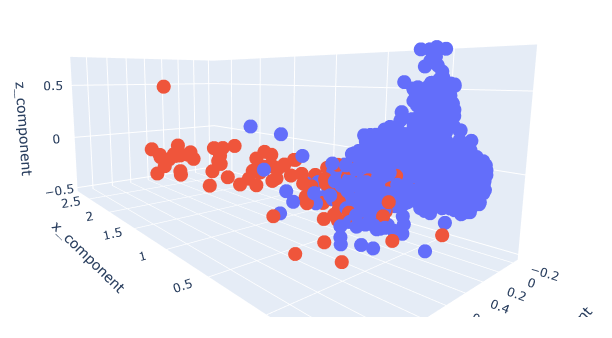
\includegraphics[width=9cm, scale=1]{images/scatter_cluster_good}
    \captionsetup{type=figure}
	\captionof{figure}{Scatter Plot Machine-2-3}
\end{center}
\begin{center}
	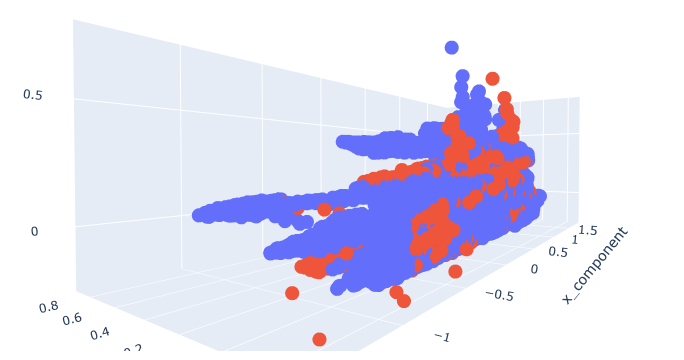
\includegraphics[width=9cm, scale=1]{images/scatter_cluster}
    \captionsetup{type=figure}
	\captionof{figure}{Scatter Plot Machine-1-7}
\end{center}

\newpage
\subsubsection{Rank Aggregation}
A questo punto ci si puo concetrare sulle varie tecniche di aggregazione. A primo impatto si puo vedere, in tabella \ref{agg-results}, come il metodo ottimale di aggregazione, che ricordiamo essere NP-Hard, produca i risultati miglori rispetto al ranking supervisionato. 
I valori medi rispetto ai dataset si aggirano intorno al range [0.4,0.6], in linea con le performance di Model Centrality e migliori rispetto a Performance on Synthetic Anomaly Injection e Clustering Cohesion. Questo vuol dire che i metodi di aggregazione riescono comunque a produrre buoni risultati nonostante le metriche surrogante non funzioni sempre bene. 
Questo tipo di aggregazione permette di avere risultati migliori quando non si ha la certezza che una sola metrica surrogata sia sufficiente. Potrebbe comunque essere utile un'analisi specifica per andare a prendere in considerazione soltanto quelle metriche surrogate, o piu nello specifico i metodi utilizzati al loro interno (rr, mv, samp, mix, scale, wander ecc), che potrebbero funzionare meglio per uno specifico dataset. 


\begin{table}[]
	\caption{\label{agg-results}Risultati di correlazione per aggregazione}
	\resizebox{\linewidth}{!}{%
		\begin{tabular}{|l||l|l|l|l||l|l|l|l||l|l|l|l|} 
			\hline
			Dataset           & \multicolumn{4}{c||}{SCORE CORRELATION} & \multicolumn{8}{c|}{RANK CORRELATION}                            \\ 
			\hline
			\multirow{2}{*}{} & \multicolumn{4}{c||}{PEARSON}           & \multicolumn{4}{c||}{KENDALL}  & \multicolumn{4}{c|}{SPEARMAN}   \\ 
			\cline{2-13}
			                & score & borda & rborda & opt   & score & borda & rborda & opt   & score & borda        & rborda & opt   \\ 
			\hline
			2\_annthyroid   & 0.795 & 0.644 & 0.394  & 0.768 & 0.486 & 0.499 & 0.382  & 0.586 & 0.550 & 0.587        & 0.331 & 0.696 \\ 
			\hline
			6\_cardio       & 0.758 & 0.589 & 0.409  & 0.597 & 0.578 & 0.416 & 0.374  & 0.550 & 0.693 & 0.545        & 0.447 & 0.572 \\ 
			\hline
			11\_donors      & 0.404 & 0.633 & 0.164  & 0.541 & 0.348 & 0.553 & 0.129  & 0.573 & 0.430 & 0.672        & 0.195 & 0.683 \\ 
			\hline
			20\_letter      & 0.595 & 0.561 & 0.436  & 0.664 & 0.493 & 0.423 & 0.418  & 0.546 & 0.606 & 0.557        & 0.406 & 0.639 \\ 
			\hline
			23\_mammography & 0.681 & 0.770 & 0.489  & 0.793 & 0.495 & 0.587 & 0.427  & 0.654 & 0.599 & 0.748        & 0.427 & 0.822 \\ 
			\hline
			27\_PageBlocks  & 0.843 & 0.753 & 0.395  & 0.860 & 0.594 & 0.551 & 0.323  & 0.659 & 0.690 & 0.713        & 0.375 & 0.822 \\ 
			\hline
			31\_satimage-2  & 0.574 & 0.761 & 0.489  & 0.730 & 0.428 & 0.559 & 0.389  & 0.630 & 0.584 & 0.736        & 0.457 & 0.816 \\ 
			\hline
			32\_shuttle     & 0.562 & 0.843 & 0.696  & 0.899 & 0.500 & 0.644 & 0.592  & 0.755 & 0.590 & 0.806        & 0.674 & 0.882 \\ 
			\hline
			38\_thyroid     & 0.623 & 0.616 & 0.367  & 0.644 & 0.477 & 0.451 & 0.390  & 0.526 & 0.536 & 0.561        & 0.334 & 0.655 \\ 
			\hline
			40\_vowels      & 0.765 & 0.813 & 0.578  & 0.807 & 0.649 & 0.632 & 0.430  & 0.661 & 0.833 & 0.816        & 0.546 & 0.858 \\ 
			\hline
			41\_Waveform    & 0.581 & 0.623 & 0.536  & 0.521 & 0.560 & 0.464 & 0.435  & 0.576 & 0.673 & 0.586        & 0.540 & 0.668 \\ 
			\hline
			machine-1-1     & 0.464 & 0.556 & 0.311  & 0.620 & 0.486 & 0.434 & 0.292  & 0.564 & 0.526 & 0.581        & 0.302 & 0.684 \\ 
			\hline
			machine-1-2     & 0.820 & 0.797 & 0.423  & 0.777 & 0.623 & 0.591 & 0.423  & 0.632 & 0.841 & 0.753        & 0.413 & 0.782 \\ 
			\hline
			machine-1-3     & 0.245 & 0.686 & 0.416  & 0.623 & 0.294 & 0.596 & 0.437  & 0.561 & 0.291 & 0.689        & 0.413 & 0.651 \\ 
			\hline
			machine-1-4     & 0.411 & 0.577 & 0.390  & 0.475 & 0.390 & 0.491 & 0.397  & 0.496 & 0.470 & 0.589        & 0.449 & 0.512 \\ 
			\hline
			machine-1-5     & 0.496 & 0.581 & 0.423  & 0.477 & 0.429 & 0.411 & 0.480  & 0.460 & 0.567 & 0.537        & 0.448 & 0.589 \\ 
			\hline
			machine-1-6     & 0.476 & 0.302 & 0.259  & 0.554 & 0.376 & 0.342 & 0.292  & 0.361 & 0.363 & 0.381        & 0.291 & 0.437 \\ 
			\hline
			machine-1-7     & 0.413 & 0.354 & 0.250  & 0.375 & 0.372 & 0.314 & 0.312  & 0.378 & 0.500 & 0.410        & 0.322 & 0.451 \\ 
			\hline
			machine-1-8     & 0.385 & 0.417 & 0.243  & 0.507 & 0.319 & 0.347 & 0.254  & 0.406 & 0.392 & 0.311        & 0.227 & 0.511 \\ 
			\hline
			machine-2-1     & 0.606 & 0.510 & 0.396  & 0.559 & 0.427 & 0.436 & 0.395  & 0.497 & 0.554 & 0.446        & 0.350 & 0.513 \\ 
			\hline
			machine-2-2     & 0.761 & 0.658 & 0.426  & 0.623 & 0.434 & 0.492 & 0.434  & 0.478 & 0.560 & 0.577        & 0.418 & 0.607 \\ 
			\hline
			machine-2-3     & 0.861 & 0.876 & 0.825  & 0.895 & 0.709 & 0.783 & 0.632  & 0.760 & 0.816 & 0.881        & 0.805 & 0.886 \\ 
			\hline
			machine-2-4     & 0.453 & 0.497 & 0.432  & 0.511 & 0.451 & 0.431 & 0.489  & 0.496 & 0.541 & 0.513        & 0.473 & 0.572 \\ 
			\hline
			machine-2-5     & 0.129 & 0.425 & 0.320  & 0.297 & 0.241 & 0.396 & 0.363  & 0.399 & 0.294 & 0.346        & 0.378 & 0.469 \\ 
			\hline
			machine-2-6     & 0.725 & 0.726 & 0.312  & 0.789 & 0.498 & 0.531 & 0.314  & 0.584 & 0.634 & 0.676        & 0.335 & 0.738 \\ 
			\hline
			machine-2-7     & 0.792 & 0.776 & 0.554  & 0.839 & 0.591 & 0.576 & 0.457  & 0.626 & 0.730 & 0.717        & 0.600 & 0.762 \\ 
			\hline
			machine-2-8     & 0.933 & 0.839 & 0.575  & 0.903 & 0.774 & 0.726 & 0.505  & 0.763 & 0.870 & 0.825        & 0.566 & 0.882 \\ 
			\hline
			machine-2-9     & 0.587 & 0.624 & 0.532  & 0.629 & 0.535 & 0.444 & 0.484  & 0.549 & 0.623 & 0.584        & 0.480 & 0.580 \\ 
			\hline
			machine-3-1     & 0.554 & 0.624 & 0.451  & 0.670 & 0.482 & 0.486 & 0.398  & 0.578 & 0.565 & 0.574        & 0.454 & 0.661 \\ 
			\hline
			machine-3-2     & 0.661 & 0.687 & 0.497  & 0.683 & 0.608 & 0.573 & 0.478  & 0.607 & 0.779 & 0.656        & 0.566 & 0.676 \\ 
			\hline
			machine-3-3     & 0.065 & 0.287 & 0.256  & 0.341 & 0.112 & 0.242 & 0.325  & 0.356 & 0.154 & 0.261        & 0.329 & 0.415 \\ 
			\hline
			machine-3-4     & 0.239 & 0.387 & 0.394  & 0.203 & 0.392 & 0.332 & 0.325  & 0.428 & 0.351 & 0.373        & 0.374 & 0.395 \\ 
			\hline
			machine-3-5     & 0.844 & 0.622 & 0.454  & 0.675 & 0.744 & 0.503 & 0.463  & 0.569 & 0.866 & 0.582        & 0.437 & 0.648 \\ 
			\hline
			machine-3-6     & 0.363 & 0.390 & 0.294  & 0.401 & 0.318 & 0.385 & 0.270  & 0.437 & 0.305 & 0.300        & 0.260 & 0.523 \\ 
			\hline
			machine-3-7     & 0.355 & 0.496 & 0.497  & 0.424 & 0.425 & 0.418 & 0.436  & 0.520 & 0.485 & 0.419        & 0.404 & 0.536 \\ 
			\hline
			machine-3-8     & 0.586 & 0.660 & 0.534  & 0.630 & 0.468 & 0.500 & 0.427  & 0.552 & 0.589 & 0.597        & 0.535 & 0.642 \\ 
			\hline
			machine-3-9     & 0.496 & 0.677 & 0.526  & 0.590 & 0.496 & 0.529 & 0.448  & 0.604 & 0.555 & 0.622        & 0.526 & 0.701 \\ 
			\hline
			machine-3-10    & 0.021 & 0.365 & 0.382  & 0.262 & 0.152 & 0.259 & 0.379  & 0.313 & 0.175 & 0.327        & 0.343 & 0.395 \\ 
			\hline
			machine-3-11    & 0.590 & 0.612 & 0.553  & 0.639 & 0.467 & 0.449 & 0.426  & 0.511 & 0.469 & 0.596        & 0.558 & 0.642 \\ 
			\hline
			AVG             & 0.552 & 0.605 & 0.433  & 0.610 & 0.467 & 0.482 & 0.401  & 0.544 & 0.555 & 0.576        & 0.430 & 0.640 \\ 
			\hline
			STD             & 0.22  & 0.154 & 0.127  & 0.177 & 0.141 & 0.115 & 0.09   & 0.107 & 0.177 & 0.156        & 0.121 & 0.138 \\
			\hline
		\end{tabular}
	}
\end{table}

\newpage
\subsubsection{Varying K}
Interessante vedere come Robust Borda, che sulla carta dovrebbe avere performance migliori, sia in verita inferiore alla sua versione standard Borda. Un motivo di cio puo stare nel fatto che ci sono modelli che sono nelle posizioni top per quanto riguarda alcune metriche surrogate ma che performano sufficientemente male in altre e vedendosi quindi penalizzate troppo.
Si puo vedere infatti, nell'immagine \ref{varying-k}, che all'aumentare del fattore K aumentano le performance di Robust Borda, fino arrivare al valore massimo con K=N, ovvero Borda normale.
Il metodo di score e' il piu semplice ma produce anche risultati relativamente scarsi. Nel nostro caso, con sole 3 metriche surrogate che vengono aggregate, l'utilizzo del metodo ottimale risulta la scelta migliore nonostante la complessita temporale sia piu alta. Se si fossero prese in considerazione piu metriche, questo approccio non sarebbe piu possibile proprio per la natura NP-Hard del problema.

\begin{figure}[t]
	\centering
	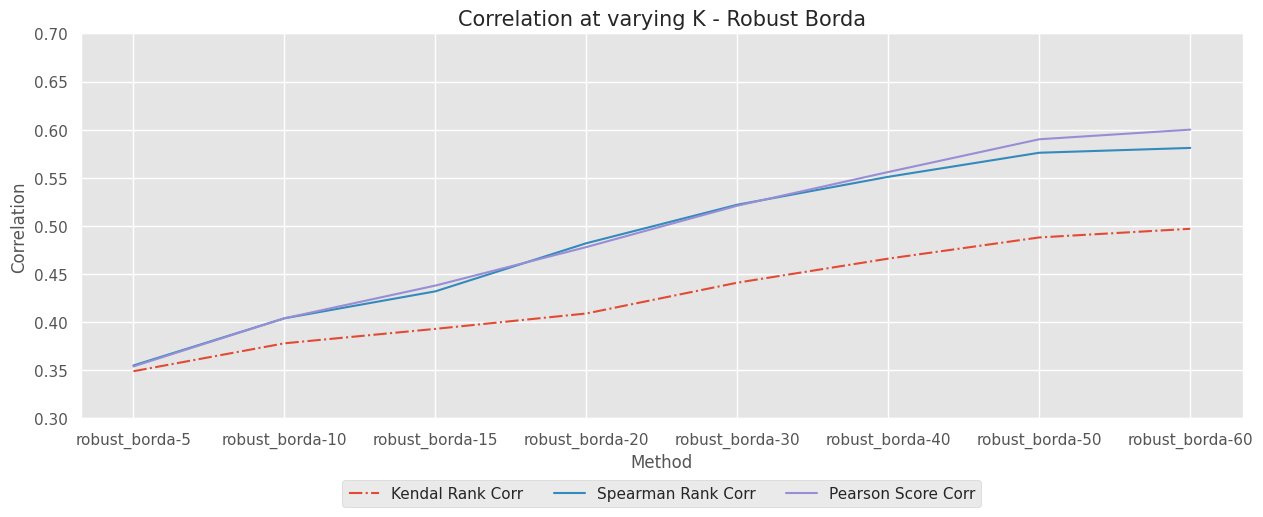
\includegraphics[width=14cm, scale=1]{images/varying-k}
	\caption{Performance di Robust Borda al variare del parametro K}
	\label{varying-k}
		
\end{figure}

\subsubsection{Ripetitivita}
Alcune metriche surrogate includono al loro interno un fattore di casualita, in particolare Sampling e tutte e 4 le tecniche di anomaly injection. Il primo metodo puo variarire ad ogni suo utilizzo in quanto per ogni sample viene scelto a caso quale modello usare come riferimento per la label. Invece i metodi di anomaly injection genereranno sempre anomalie differenti in quanto sia la posizione che il magnitudo di anomalia cambia ogni volta.
Per questo motivo e' stata fatta anche un'analisi andando a ripetere il Model Selection su due dataset per 5 volte.
Nell'immagine \ref{score-box}  e' possibile vedere un Box Whisker Plot sugli score prodotti da Model Selection per ognuna delle metriche e metodi. Alcuni di questi non includono casualita come Round Robin, Majority Vote, Score Correlation e Score Clustering, di conseguenza il valore e' uguale ad ogni iterazione. Al contrario gli altri vedono differire il valore ad ogni iterazione, chi piu chi meno. In generale, vi e' un range che varia di circa 0.05 punti.

\begin{figure}[t]
	\centering
	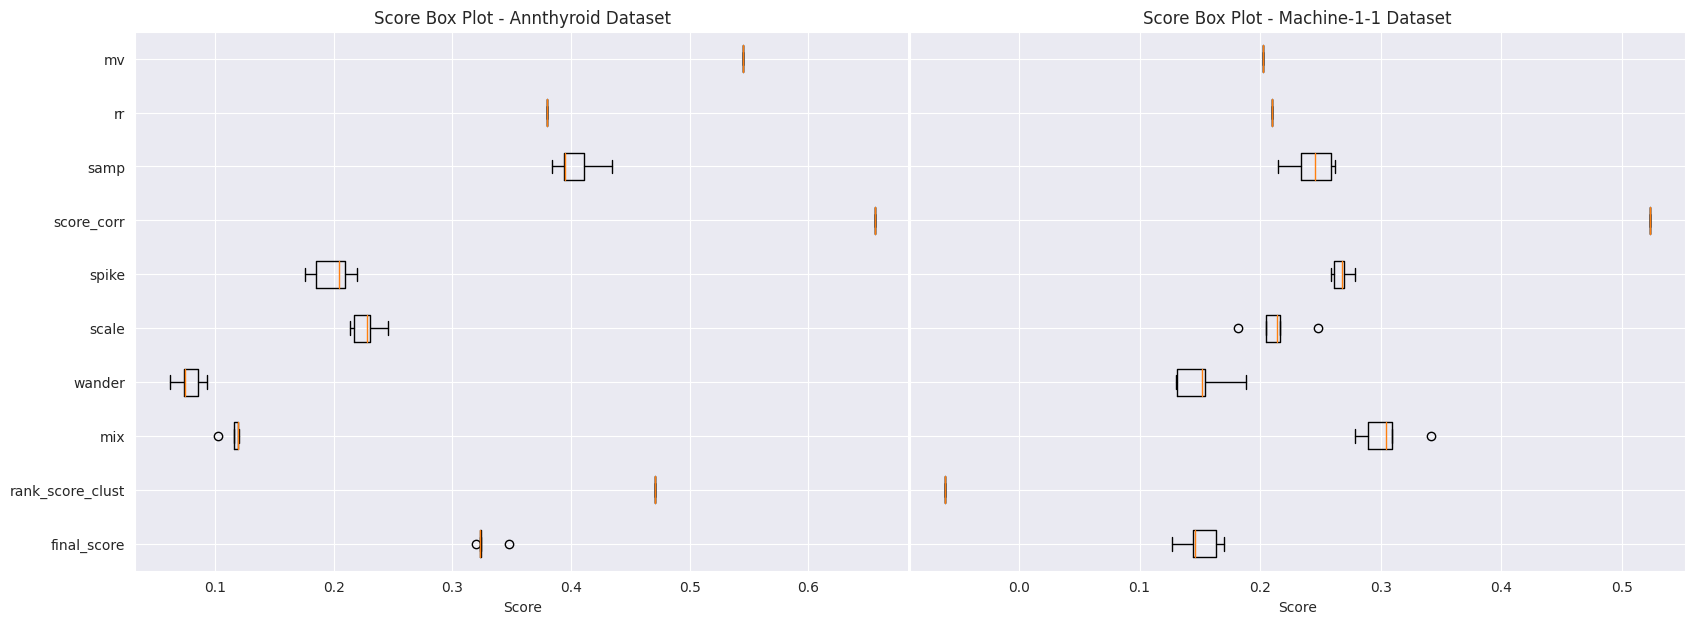
\includegraphics[width=15cm, scale=1]{images/score_box}
	\caption{Score Box Plot}
	\label{score-box}
	
\end{figure}

Queste differenze negli score vanno anche ad impattare poi il coefficiente di correlazione Kendall rispetto al Ranking Supervisionato. Anche qui, come prima, le differenze sono esigue ma sempre presenti; immagine \ref{kendall-box}.

\begin{figure}[t]
	\centering
	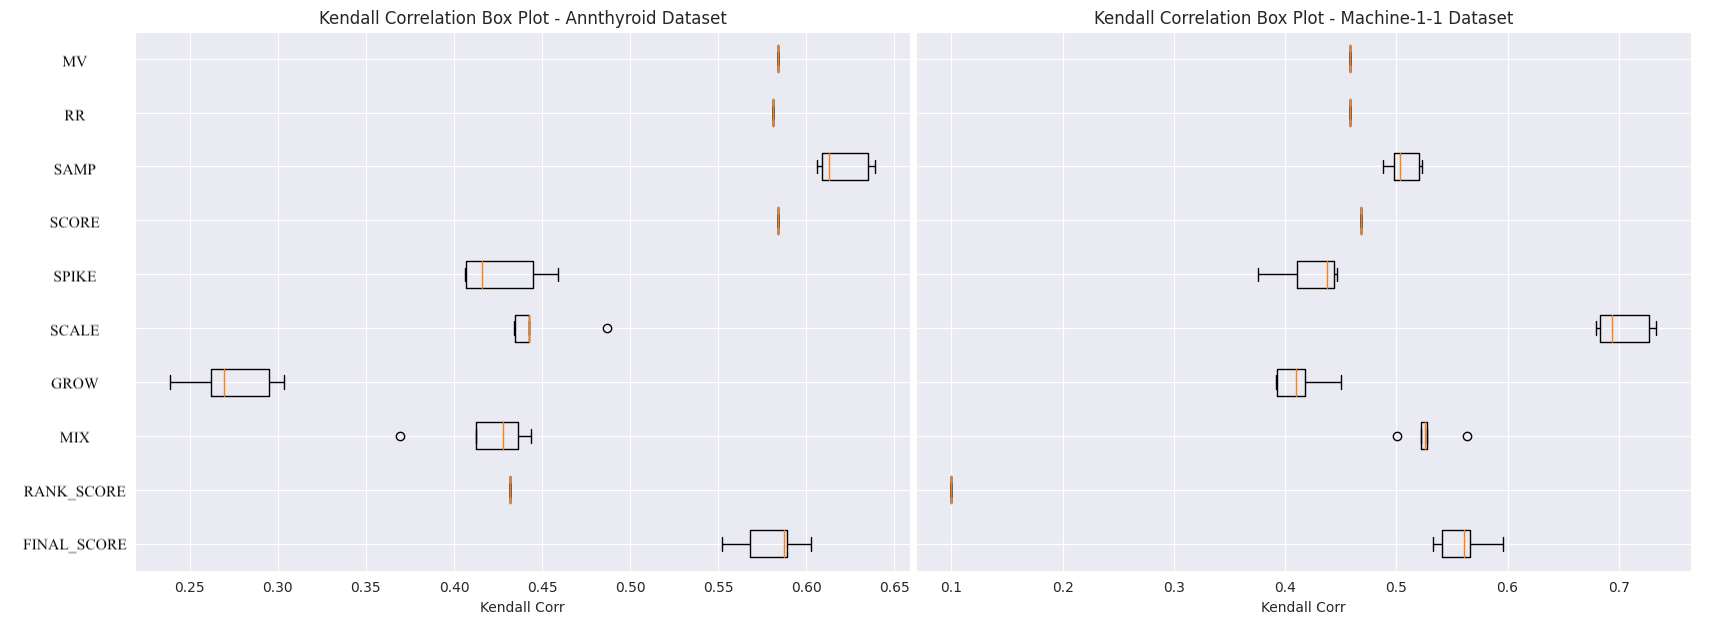
\includegraphics[width=15cm, scale=1]{images/kendall_box}
	\caption{Kendall Correlation Box Plot}
	\label{kendall-box}
		
\end{figure}


\subsubsection{Quantile Interesection}
Oltre a valutare le performance sullo score di correlazione tra il ranking non supervisionato e quello supervisionato, puo risultare utile cambiare punto di vista e comparare i ranking in se.
Per questa valutazione sono stati ordinati i ranking per il loro score e poi sono stati divisi in 2 o 4 quantili. Successivamente viene calcolata l'interesezione del quantile di un ranking con il corrispondente del secondo ranking.
Come mostrato nella figura \ref{quantile-intersection}, si puo notare come dividendo in 2 quantili, l'intersezione sia quasi perfetta, segno che l'algoritmo di model selection sa distinguere i modelli piu performanti con quelli meno performanti.
Passando a 4 quantili gli score di intersezione scendono, mostrando come il Model Selection faccia piu fatica a trovare una corrispondenza perfetta. Si puo comunque notare come il quarto quantile sia stato trovato con un'alta confidenza.
Possiamo quindi concludere che mentre il model Selection non supervisionato non sia molto preciso nel trovare i modelli che siano effettivamente i migliori, e' in grado di escludere abbastanza bene quelli peggiori. A confermare questa ipotesi il calcolo dei quantile interserction con soltanto due bin, producendo uno score di interessezione di \(0.8\)

\begin{figure}[t]
	\centering
	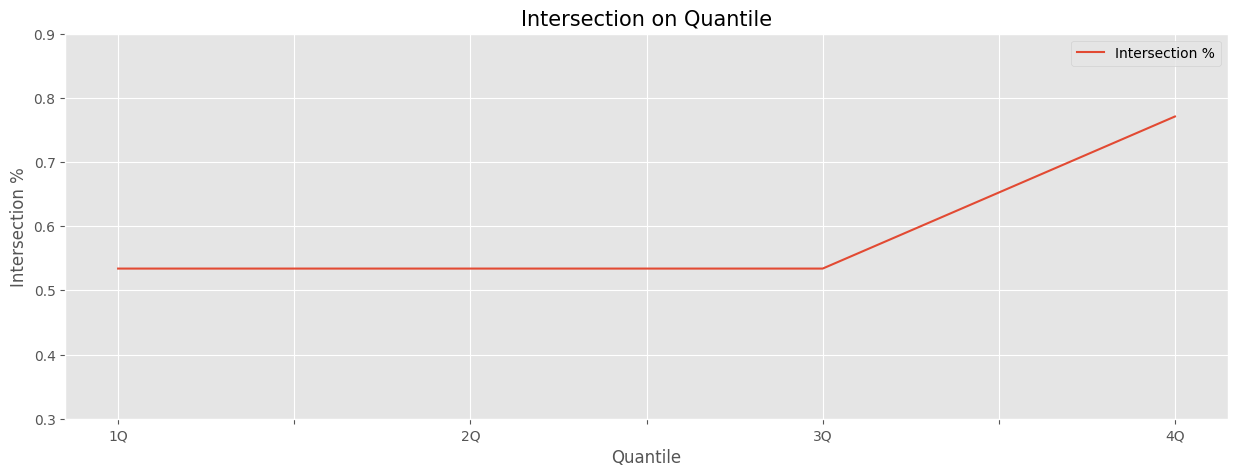
\includegraphics[width=14cm, scale=1]{images/4quantile}
	\caption{Intersezione tra quantili}
	\label{quantile-intersection}
		
\end{figure}


\newpage
\section{SKF Results}
Il progetto di tesi e' nato da una collaborazione tra Alten e SKF quindi una parte dedicata a quest'ultima e' necessaria. Come introdotto nel capitolo \ref{chap:skf} pero, i dati prodotti dai sensori installati sui macchinari della catena di montaggio non sono sufficientemente completi per riuscire a fornire una valutazione completa dell'algoritmo di Model Selection. La mancanza di labels e di uno storico delle manutenzioni effettuate in aggiunta al fatto che non tutte le macchine sono mappate dai sensori, rende complicato valutare i modelli di Anomaly Detection. La presenza dei dati MVM aiuta poco alla causa per tre motivi: (1) non tutte le macchine hanno sensori installati, (2) la frequenza con la quale vengono registrati i dati CoMo e troppo bassa e (3) la correlazione tra i valori dei sensori e la qualita finale non e' certo da dare per scontata. Potrebbero esserci fattori aggiuntivi come la qualita del materiale utilizzato per la produzione oppure anche problemi ai macchinari che non vengono captati dai sensori. 
Nonostante cio, viene svolta una valutazione usando MVM come riferimento. Prima viene eseguito l'algoritmo di Model Selection non supervisionato sul dataset di uno specifico macchinario andando a produrre una lista di ranking e ottenendo cosi il modello in prima posizione, successivamente viene usato questo per andare a fare la prediction sui dato sempre dello stesso macchinario. Infine si utilizzano i dati di MVM per:
\begin{itemize}
	\item Calcolare il numero di volte in cui un cuscinetto a sfera supera la soglia della banda A per la classe Q1 nell'intervallo di 10 minuti e paragonare questi numeri tra i time-step segnalati come anomali dal modello con i time-step segnalati come normali.
	\item Calcolare la qualita media per ogni intervallo di 10 minuti e misurare la correlazione tra la qualita con le label generate dal modello per ogni intervallo.
\end{itemize}
L'assunzione forte che e' stata fatta e' che situazione anomale di un macchinario portino a qualita del prodotto finito piu bassa, ovvero a valori di MVM piu alti. Quello che si spera di ottenere e' vedere questa assunzione all'atto pratico, ovvero con valori di MVM mediamente piu alti(qualita piu bassa) per quei punti considerati anomali da un modello rispetto ai punti considerati normali.


\subsection{Dataset}
I dataset di SKF sono stati introdotti e dettagliati nel capitolo \ref{chap:skf}. Per questa fase di valutazione vengono usati sia i dati di MVM, piu nello specifico viene usata la banda A riguardante gli errori geometrici, ovvero il gridining. Questo perche si e' deciso di concentrarsi esclusivamente sul un macchinario che, per motivi di privacy, chiameremo M1. Questo macchinario e' il primo nella linea di produzione ed effettua il grinding, quindi direttamente interessato alla banda A.
Per la fase di training e' stato scelto il periodo che va da gennaio a marzo 2022 in quanto i dati in quel periodo risultavano i piu puliti ed i piu stabili da un punto di vista di oscillazioni o data change. Mentre per la fase di prediction viene usato come riferimento il periodo maggio-giugno 2022.



\subsection{Thresholding}
Prima di procedere al training del modello e' necessario avere un riferimento sulla percentuale di anomalie nel dataset. A questo scopo e' stato utilizzato il metodo GammaY introdotto nel capitolo \ref{chap:methods}.
Questo algoritmo riceve in input la stessa lista di modelli candidati usati poi nel model selection, e dopo essere stati allenati sul dataset di training senza andare ad indicare il fattore di contaminazione sono stati usati gli output score prodotti da ognuno di questi per computare la distribuzione di probabilita multivariata delle anomalie.
Il risultato prodotto da questa tecnica di trhesoldin e' 0.05, ovvero il 5\% di punti vengono considerati anomali. Un dato ragionevole confermato da un analisi manuale dei dati.


\subsection{Risultati}
L'algoritmo di Model Selection, eseguito sul dataset del macchinario M1 utilizzando come modelli la medesima lista utilizzata con i dataset di benchmark, ha prodotto i seguenti risultati:


\begin{table}[H]
	\begin{minipage}{.5\textwidth}
		\centering
		\resizebox{\columnwidth}{!}{%
			\begin{tabular}{|l|l|l|l|l|l|} 
				\hline
				\textbf{\#} & \textbf{Model} & \textbf{RR} & \textbf{MIX} & \textbf{CC} & \textbf{F.Score} \\ 
				\hline
				1           & KDE            & 0.544       & 0.391        & 0.549       & 0.990            \\ 
				\hline
				2           & CBLOF\_4       & 0.539       & 0.388        & 0.501       & 0.988            \\ 
				\hline
				3           & MCD            & 0.508       & 0.483        & 0.530       & 0.955            \\ 
				\hline
				4           & IForest\_200   & 0.509       & 0.320        & 0.554       & 0.938            \\ 
				\hline
				5           & OCSVM\_poly    & 0.452       & 0.386        & 0.542       & 0.920            \\ 
				\hline
				6           & OCSVM\_sig     & 0.452       & 0.384        & 0.542       & 0.919            \\ 
				\hline
				7           & PCAODetector   & 0.552       & 1.000        & 0.510       & 0.901            \\ 
				\hline
				8           & KPCA           & 0.548       & 0.335        & 0.528       & 0.899            \\ 
				\hline
				9           & PCA            & 0.552       & 0.077        & 0.510       & 0.893            \\ 
				\hline
				10          & KNN\_10        & 0.562       & 0.286        & 0.474       & 0.830            \\
				\hline
			\end{tabular}
			}\captionof{table}{Top 10}
	\end{minipage}
	\begin{minipage}{.5\textwidth}
		\centering
		\resizebox{\columnwidth}{!}{%
			\begin{tabular}{|l|l|l|l|l|l|} 
				\hline
				\textbf{\#} & \textbf{Model} & \textbf{RR} & \textbf{MIX} & \textbf{CC} & \textbf{F.Score} \\ 
				\hline
				70          & SO\_GAAL       & 0.005       & 0.029        & 0.314       & 0.030            \\ 
				\hline
				69          & Telemanom      & 0.090       & 0.997        & 0.237       & 0.030            \\ 
				\hline
				68          & DeepSVDD       & 0.214       & 0.120        & 0.348       & 0.035            \\ 
				\hline
				67          & ALAD           & 0.071       & 0.092        & 0.375       & 0.067            \\ 
				\hline
				66          & SOS            & 0.218       & 0.143        & 0.391       & 0.098            \\ 
				\hline
				65          & SOS\_7         & 0.228       & 0.143        & 0.370       & 0.118            \\ 
				\hline
				64          & FeatureBagging & 0.335       & 0.024        & 0.406       & 0.127            \\ 
				\hline
				63          & LOF            & 0.337       & 0.065        & 0.390       & 0.136            \\ 
				\hline
				62          & PCAODetector   & 0.103       & 0.997        & 0.394       & 0.136            \\ 
				\hline
				61          & ABOD           & 0.423       & 0.054        & 0.391       & 0.139            \\
				\hline
			\end{tabular}}\captionof{table}{Worst 10}
	\end{minipage}
\end{table}




Sono proposti i primi 10 e gli ultimi 10 modelli con i relativi score finali. Le metriche surrogate utilizzate sono state (1) Round Robin per Model Centrality, (2) Mix per Performance on Synthethic Anomaly Injection e (3) Clustering Cohesion. La tecnica di aggregazione utilizzata e' stato il metodo ottimale di Kenedy-Young.
Il primo modello e' KDE, ovvero Kernel Density Estimation ed in generale i metodi di Machine Learning hanno uno score piu alto di quelli Deep Learning. Situazione rimarcata dal fatto che per le ultime 10 posizioni sono presenti 4 metodi di Deep Learning. Una spiegazione ha questo fenomeno risiede nel fatto che questi modelli hanno score di Model Centrality e Anomaly Injection molto bassi. Eccezione per Telemanom che riesce a riconoscere quasi perfettamente tutte le anomalie sintetiche iniettate. Gli Score di Clustering Cohesion vanno anche questa volta a favorire metodi di Machine Learning, anche se in misura piu lieve. Infatti i modelli come DeepSVDD o ALAD riescono a  raggiungere punteggi intorno al 0.4, in linea con i migliori.
Model Centrality va sicuramente a favorire quei modelli che producono output simile tra di loro, implicando una forte varianza dei risultati sulla base di quali modelli candidati vengono passati all'algoritmo di Model Selection. Potrebbe essere il caso che i modelli di Deep Learning siano effettivamente i migliori, ma essendo pochi rispetto al numero totale di modelli considerati, il loro punteggio di Model Centrality va abbassandosi. In questi casi, un'analisi grafica delle anomalie rilevate puo risultare utile.

\subsubsection{Anomalie Rilevate}
Attraverso un grafico a linee con barre verticali per rappresentare i timestep rilevati come anomalia, possiamo notare nella figura \ref{kde} come KDE, ovvero il miglior modello, riesca a riconoscere bene i punti di spike o gli intervalli di spike in cui certi sensori raggiungono valori sufficientemente distanti da un comportamento standard. Al contrario, figura \ref{worst_clf}, Telemanom raggruppa tutti i punti anomali in un unico intervallo continuo nonostante ci siano dei timestep che non presentino, ad occhio, un comportamento anomalo.

\begin{figure}[t]
	\centering
	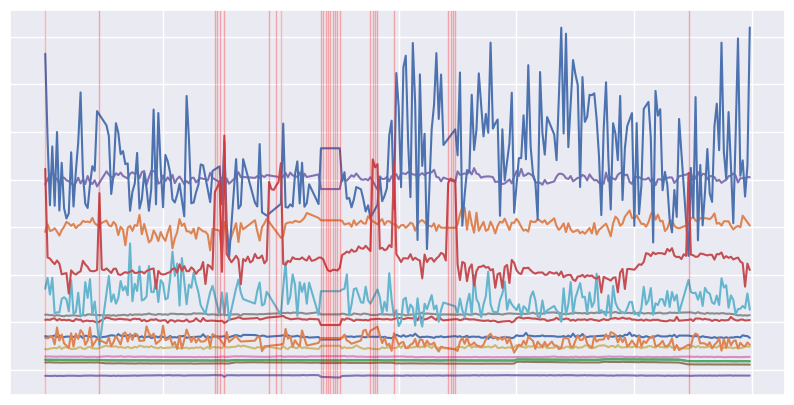
\includegraphics[width=14cm, scale=1]{images/kde}
	\caption{Anomalie Rilevate da KDE}
	\label{kde}
	
\end{figure}

\begin{figure}[t]
	\centering
	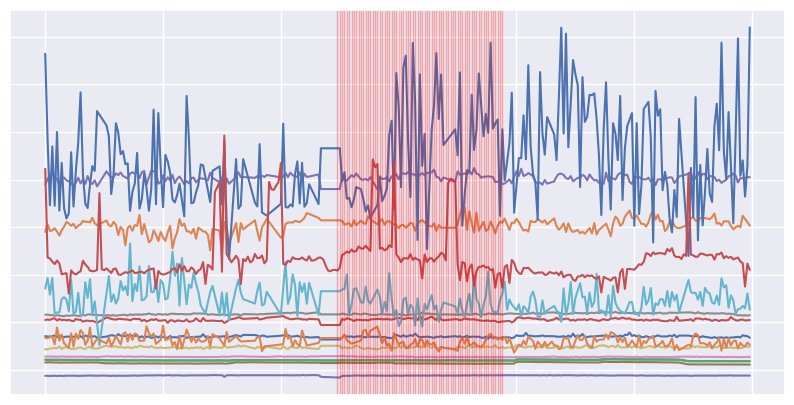
\includegraphics[width=14cm, scale=1]{images/worst_clf}
	\caption{Anomalie Rilevate da Telemanom}
	\label{worst_clf}
	
\end{figure}

Passando ad un plot scatter dopo aver ridotto la dimensionalita dei punti a 2 dimensioni tramite PCA, possiamo notare in figura \ref{kde_scatter} due cluster principali con punti sparsi nel mezzo. I punto anomali trovati da KDE si trovano principalmente nel cluster piu piccolo a destra e nei punti sparsi nel piano. Mentre il cluster blu in centro risulta ben omogeneo.
Telemanom invece labella come anomali principalmente i punti del cluster di sinistra, risultando in una separazione meno chiara, figura \ref{worst_clf_scatter}.
Ovviamente non si ha la certezza che il cluster di destra sia effettivamente composto da tutti punti anomali, ma chiaramente un comportamento fuori dal normale c'e' in quanto la stragrande maggioranza dei dati, risiedenti nel cluster di sinistra, possiede valori molto diversi.


\begin{figure}[t]
	\centering
	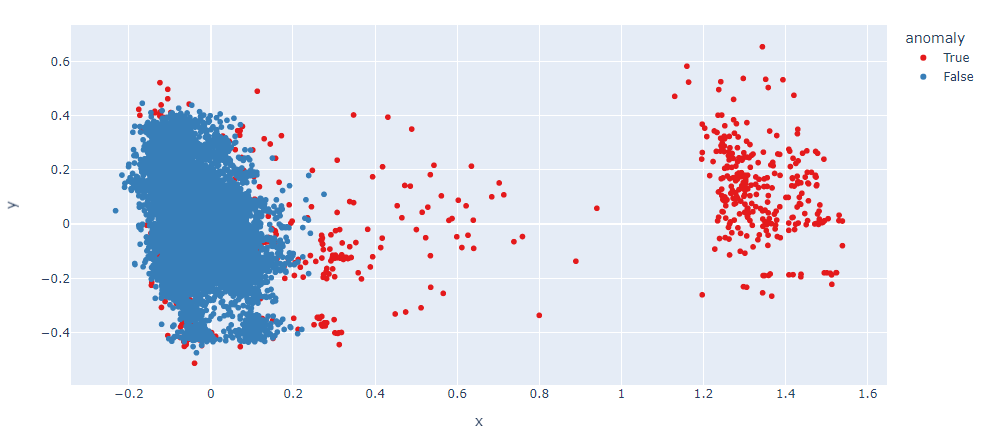
\includegraphics[width=14cm, scale=1]{images/kde_scatter}
	\caption{Scatter Plot delle anomalie KDE}
	\label{kde_scatter}
		
\end{figure}




\begin{figure}[t]
	\centering
	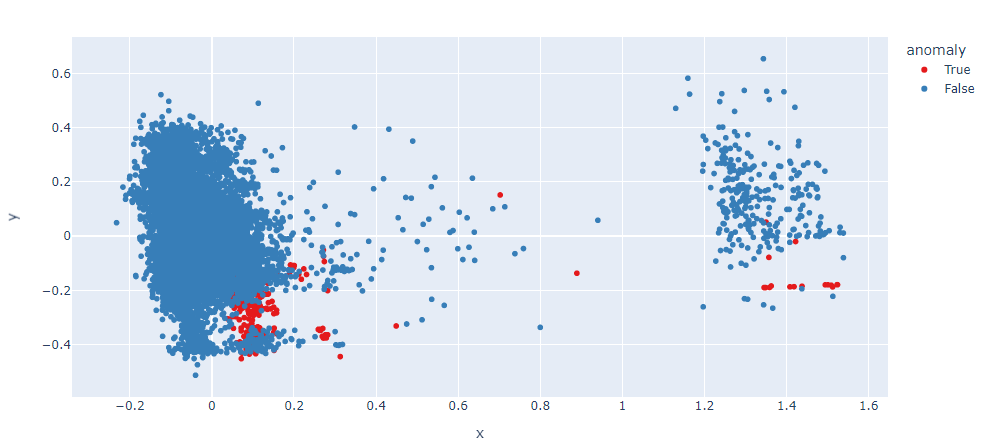
\includegraphics[width=14cm, scale=1]{images/worst_clf_scatter}
	\caption{Scatter Plot delle anomalie Telemanom}
	\label{worst_clf_scatter}
		
\end{figure}

\subsubsection{Confronto Qualita}
Puo essere utile un confronto tra le anomalie rilevate e la qualita registrata in quei timestep. Come anticipato piu volte, la qualita non e' da considerarsi un perfetto indicatore delle anomalie: 
\begin{itemize}
	\item La qualita viene registrata ogni due secondi mentre i dati CoMo ogni 5 minuti. Di conseguenza la qualita viene aggregata con una media, andando a nascondere, nel calcolo aggregato, i valori piu alti che sono anche i piu rari. Usare altre tecniche di aggregazione come Min o Max non e' immediato in quanto avrebbe poi favorito troppo o troppo poco la presenza di valori di qualita' estremi.
	\item Analizzando un solo macchinario non e' possibile avere una situazione completa della linea di produzione, ma anche analizzando tutti i macchinari insieme non e' certo che la qualita' sia correllata al 100\% con i dati CoMo. Ci possono essere fattori come la qualita del materiale o degli oli, o altri movimenti dei macchinari non registrati che impattano la qualita. Producendo quindi valori di qualita bassa nonostate registrazioni CoMo nella norma. Oppure il contrario, ovvero registrazioni CoMo anomale ma che non impattano la qualita.
\end{itemize}


Nelle prossime due immagini possiamo vedere lo stesso scatter plot di prima, ma andando a colorare i punti sulla base della correlazione tra punti rilevati come anomali da un modello, in questo caso prima KDE poi Telemanom, e i punti registrati come bassa qualita. Le correlazioni sono cosi spiegate:
\begin{itemize}
	\item \textit{true positive} indica che il punto e' rilevato sia come anomalo che di bassa qualita
	\item \textit{true negative} indica che il punto e' rilevato sia come non anomalo che di qualita normale
	\item \textit{false negative} indica che il punto e' rilevato come non anomalo ma la qualita e' bassa
	\item \textit{false positive} indica che il punto e' rilevato come anomalo ma la qualita e' normale
\end{itemize}

L' immagine \ref{kde_quality} rappresenta lo scatter con KDE, la maggior parte dei punti del cluster di sinista viene correttamente identificato come true-negative ma sono presenti discreto numero di false negative non banale. Il cluster di destra, cosi come i punti sparsi nel mezzo, vengono identificati per circa meta come false positive e meta come true positive.
\begin{figure}[t]
	\centering
	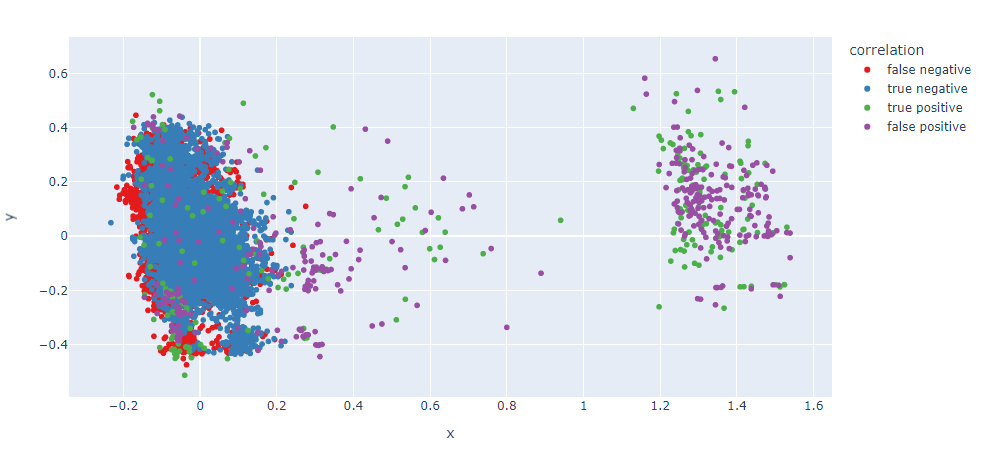
\includegraphics[width=14cm, scale=1]{images/correlation_ssb1_quality_plot.png}
	\caption{Scatter Plot Correlazione Qualita KDE}
	\label{kde_quality}
\end{figure}

Con Telemanom, immagine \ref{worst_clf_quality} la situazione non e' migliore, in generale e' presente confusione nell'identificazione dei punti con qualita bassa.


\begin{figure}[t]
	\centering
	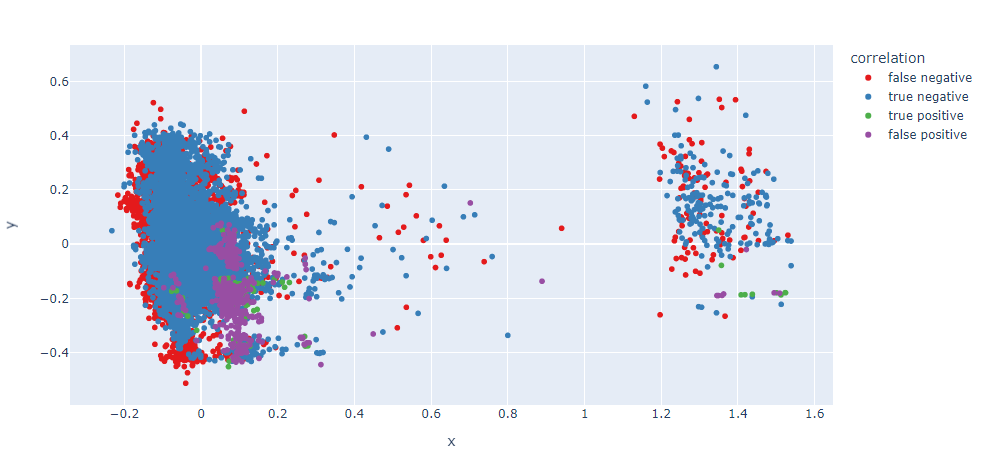
\includegraphics[width=14cm, scale=1]{images/worst_correlation_ssb1_quality_plot}
	\caption{Scatter Plot Correlazione Qualita Telemanom}
	\label{worst_clf_quality}
\end{figure}

La conferma arriva dalle matrici di confusione. Sia KDE che Telemanom non riescono a trovare punti che siano effettivamente di qualita bassa:



\begin{table}[H]
	\begin{minipage}{.5\textwidth}
		\centering
		\resizebox{\columnwidth}{!}{%
			\begin{tabular}{|l|l|l|}
				\hline
				                  & \textbf{Real Positive} & \textbf{Real Negative} \\ \hline
				\textbf{Positive} & 238 (0.05)             & 372 (0.05)             \\ \hline
				\textbf{Negative} & 4648 (0.95)            & 6885 (0.95)            \\ \hline
			\end{tabular}
			}\captionof{table}{KDE Confusion Matrix}
	\end{minipage}
	\begin{minipage}{.5\textwidth}
		\centering
		\resizebox{\columnwidth}{!}{%
			\begin{tabular}{|l|l|l|}
				\hline
				                  & \textbf{Real Positive} & \textbf{Real Negative} \\ \hline
				\textbf{Positive} & 177 (0.04)             & 430 (0.06)             \\ \hline
				\textbf{Negative} & 4709(0.96)             & 6827 (0.94)            \\ \hline
			\end{tabular}}\captionof{table}{Telemanom Confusion Matrix}
	\end{minipage}
\end{table}


\subsubsection{Confronto Qualita - Alternative}
Si potrebbe tentare di risolvere i due problemi elencati ad inizio paragrafo andando a cambiare approccio per l'analisi della correlazione.
Per il primo di questi, ovvero il problema della media di tutte le registrazioni di qualita in un dato intervallo di 10 che va a nascondere eventuali registrazioni piu rare in cui la qualita e' bassa, si puo andare a contare il numero di registrazioni, sempre all'interno di ogni intervallo, che superano la soglia Q1 per la banda A.
I risultati ottenuti sono riportati nella tabella \ref{quality_count}.

\begin{table}[]
	\centering
	\begin{tabular}{|l|ll|ll|}
		\hline
		\multirow{2}{*}{}       & \multicolumn{2}{l|}{\textbf{Punti Normali}} & \multicolumn{2}{l|}{\textbf{Punti Anomali}} \\ \cline{2-5} 
		                        & \multicolumn{1}{l|}{Telenamom} & KDE & \multicolumn{1}{l|}{Telemanom} & KDE \\ \hline
		\textbf{Banda A}        & \multicolumn{1}{l|}{19}        & 19  & \multicolumn{1}{l|}{14}        & 19  \\ \hline
		\textbf{Tutte le bande} & \multicolumn{1}{l|}{87}        & 85  & \multicolumn{1}{l|}{72}        & 86  \\ \hline
	\end{tabular}
	\caption{\label{quality_count}Media MVM sopra-soglia per intervallo}
\end{table}

Il numero medio di registrazioni che superano la soglia Q1 della banda A all'interno degli intervalli classificati come normali da KDE sono 19, lo stesso per gli intervalli classificati come anomali. Facendo anche un conteggio tenendo in considerazione tutte le registrazione che superano la soglia Q1 di qualsiasi banda (A,B,C e D), i risultati sono 85 per i punti normali e 86 per quelli anomali. Questi risultati implicano che non c'e' nessuna correlazione tra qualita bassa e punti anomali. 
Questo esperimento e' stato fatto anche usando Telemanom ed anche qui i risultati confermano il trend.

Per quanto riguarda il secondo punto, ovvero il problema di considerare solamente un macchinario, si e' pensato di andare a eseguire l'algoritmo di Anomaly Detection su tutti i macchinari di cui si hanno i dati della linea di produzione e aggregare insieme le label per ogni timestep.
In questo esperimento, i dati hanno bisogno di una fase di processing aggiuntiva, ovvero e' necessario allineare le registrazioni di tutti i macchinari tenendo in considerazione il tempo che impiega il cuscinetto a sfera a spostarsi lungo la linea di montaggio. In un esempio, ipotizzando tre macchine di cui la terza e' MVM ed un cuscinetto a sfera che parte dalla linea di montaggio a tempo $t$, la prima macchina esegue la registrazione su quel cuscinetto a sfera a tempo $t$, la seconda a tempo $t+1$ e la terza a tempo $t+2$. Per allineare le registrazioni viene quindi rimossa un'unita temporale dalle registrazioni del secondo macchinario e 2 unita' dalle registrazioni del terzo macchinario. Cosi facendo si crea un'istantanea delle registrazioni per ogni cuscinetto a sfera. Questo procedimento e' simile a quello svolto per le valutazioni precedenti, con la differenza che in questo caso si aveva soltato il macchinario M1 ed MVM, di conseguenza solamente i dati MVM erano da traslare.
Allineati i dati e' necessario aggregare le label di ogni macchinario per ogni timestep. E' stata scelto di applicare un approccio del tipo \textit{almeno uno}, ovvero se il modello di AD trova un'anomalia per un dato macchinario e per un dato timestep, quel timestep risultera anomalo. 
Purtroppo pero' anche con questo approccio la corrispondenza tra anomalie e qualita e' bassa, inoltre eseguendo l'algoritmo di AD su tutti e 10 i macchinari a disposizione e aggregando con il metodo \textit{almeno uno}, potenzialmente il numero di anomalie rilevate viene moltiplicato per 10, passando da un 5\% ad un 50\%. Questo fa lievitare i numeri di false positive a dismisura. Sia il plot scatter, figura \ref{quality_all_machines} che la confusion matrix, tabella \ref{cm_quality_all}, sono stati posti per visualizzazione.

\begin{figure}[t]
	\centering
	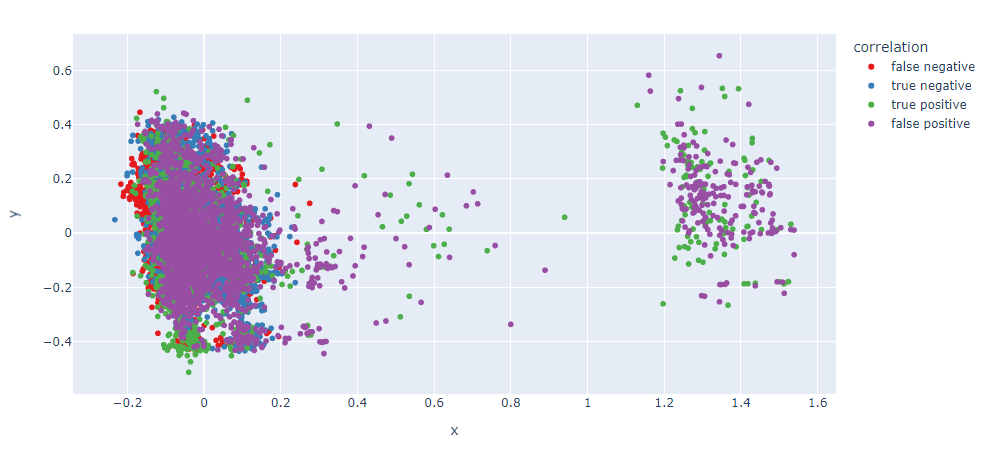
\includegraphics[width=14cm, scale=1]{images/correlation_all_quality_plot.png}
	\caption{Correlazione KDE su tutti i macchinari}
	\label{quality_all_machines}
\end{figure}

\begin{table}[]
	\centering
	\begin{tabular}{|l|l|l|}
		\hline
		                  & \textbf{Real Positive} & \textbf{Real Negative} \\ \hline
		\textbf{Positive} & 1510 (0.31)            & 2750 (0.37)            \\ \hline
		\textbf{Negative} & 3376 (0.69)            & 4507 (0.62)            \\ \hline
	\end{tabular}
	\caption{\label{cm_quality_all}Confusion Matrix KDE su tutti i macchinari}
	
\end{table}

\subsubsection{Conclusione}
In conclusione, valutare in modo automatico le performance di un modello di Anomaly Detection su SKF e' di fatto impossibile. Sarebbero necessari le registrazioni di almeno tutti i machinari della linea e frequenza di registrazione ogni 2 secondi in modo da pareggiare la frequenza di MVM. A questo punto un'analisi piu accurata sulla relazione tra MVM e CoMo puo essere svolta, ma anche in questo caso non e' detto che ci sia correlazione perfetta.
L'unico modo per valutare quindi il modello prodotto da Model Selection e' quello di portare in produzione una dashboard con PowerBI, in modo da notificare gli operatori i momenti di anomalia e ricevere feedback di conseguenza sulla precisione del modello.
Una trattazione sul ciclo di deploy e distribuzione viene fatta nel capitolo successivo.